\documentclass[12pt,a4paper,oneside]{report}

% --- PACOTES ---
\usepackage[utf8]{inputenc}
\usepackage[T1]{fontenc}
\usepackage[brazil]{babel}
\usepackage{helvet}
\renewcommand{\familydefault}{\sfdefault}
\usepackage{indentfirst}
\usepackage{setspace}
\usepackage[top=3cm,bottom=2cm,left=3cm,right=2cm]{geometry}
\usepackage{xcolor}
\usepackage{titlesec}
\usepackage{enumitem}
\usepackage{booktabs}
\usepackage{graphicx}
\usepackage{float}
\usepackage{tocloft}
\usepackage[hidelinks]{hyperref}
\usepackage{xurl}
\usepackage[num]{abntex2cite}

% --- CORES ---
\definecolor{pucblue}{RGB}{0, 51, 102}

% --- TÍTULOS ---
\titleformat{\chapter}[display]
  {\normalfont\bfseries\color{pucblue}}{\chaptertitlename\ \thechapter}{10pt}{\Huge}
\titleformat{\section}
  {\normalfont\large\bfseries\color{pucblue}}{\thesection}{1em}{}
\titleformat{\subsection}
  {\normalfont\normalsize\bfseries}{\thesubsection}{1em}{}

% --- SUMÁRIO ---
\renewcommand{\cftchapfont}{\bfseries\color{pucblue}}
\renewcommand{\cftchapleader}{\cftdotfill{\cftdotsep}}

\begin{document}

% --- CAPA ---
\begin{titlepage}
    \begin{center}
        \large\textbf{\uppercase{Pontifícia Universidade Católica de Minas Gerais}}\\[0.2cm]
        \large\textbf{\uppercase{Sistemas de Informação}}\\[4cm]
        
        \huge\textbf{\color{pucblue}Projeto de Infraestrutura de Redes:\\ Rede Hospitalar Cuidar}\\[0.5cm]
        \large\textit{Documento de Planejamento e Implementação}\\[3cm]
        
        
            \textbf{Grupo de Trabalho:}\\
            \small
            Athos Geraldo Salomon Dolabela da Silveira\\
            Bernardo Elias Renttins Vasconcelos de Sousa\\
            Fabrício Junio da Silva\\
            Henrique Fadel Carvalho\\
            Igor de Oliveira Martins dos Santos\\
            Pedro Tolentino Gontijo
        
        
        \vfill
        \large\textbf{Belo Horizonte}\\
        \large\textbf{2026}
    \end{center}
\end{titlepage}

% --- SUMÁRIO ---
\tableofcontents
\setstretch{1.5}

% ============================================================
% ETAPA 1
% ============================================================
\chapter{Etapa 1 --- Planejamento e Prototipação}

\section{Gestão e Organização do Projeto}

\subsection{Definição do Tema e Cenário}
O projeto foca na \textbf{Rede Hospitalar Cuidar}, uma instituição de saúde com matriz em Belo Horizonte e unidades remotas (Secretaria e três UPAs). O cenário exige alta disponibilidade e segmentação, dado o tráfego de dados sensíveis e a necessidade de comunicação ininterrupta para prontuários eletrônicos.

\subsection{Responsabilidades e Colaboração}
Para atender à gestão da comunicação e colaboração, o grupo utilizou ferramentas como Microsoft Teams e WhatsApp para alinhamento síncrono e assíncrono.
\begin{itemize}[label=\color{pucblue}$\bullet$]
    \item \textbf{Igor e Pedro:} Planejamento de sub-redes (CIDR), NAT e lógica de serviços.
    \item \textbf{Henrique:} Implementação técnica e nomenclatura no Cisco Packet Tracer.
    \item \textbf{Bernardo e Athos:} Gestão de ativos, custos e planilhas de inventário.
    \item \textbf{Fabrício:} Redação técnica e revisão das normas de documentação.
\end{itemize}

\subsection{Cronograma de Dedicação}
\begin{center}
\small
\begin{tabular}{ll}
\toprule
\textbf{Data} & \textbf{Tarefa} \\ \midrule
09/02 a 28/02 & Estudo dos microfundamentos e definição do cenário. \\
01/03 a 15/03 & Elaboração do inventário detalhado e cálculos de tráfego. \\
16/03 a 24/03 & Desenvolvimento do protótipo e testes de conectividade (Ping). \\
25/03 a 28/03 & Ajustes de nomenclatura conforme feedback e entrega final. \\ \bottomrule
\end{tabular}
\end{center}

\section{Arquitetura Lógica e Endereçamento}

\subsection{Divisão por CIDR e NAT}
A rede utiliza o bloco privado \texttt{10.0.0.0/8}, segmentado para otimizar o domínio de broadcast e aumentar a segurança.
\begin{center}
\footnotesize
\begin{tabular}{llll}
\toprule
\textbf{Unidade} & \textbf{Faixa de Rede} & \textbf{Gateway} & \textbf{Servidor Principal} \\ \midrule
Matriz     & 10.10.0.0/24 & 10.10.0.1 & SRV-BH-PRONTUARIO (10.10.0.10) \\
Secretaria & 10.20.0.0/24 & 10.20.0.1 & SRV-SEC-ADMIN (10.20.0.10) \\
UPA 1      & 10.30.0.0/24 & 10.30.0.1 & SRV-UPA1-LOCAL (10.30.0.10) \\
UPA 2      & 10.40.0.0/24 & 10.40.0.1 & SRV-UPA2-LOCAL (10.40.0.10) \\
UPA 3      & 10.50.0.0/24 & 10.50.0.1 & SRV-UPA3-LOCAL (10.50.0.10) \\
\bottomrule
\end{tabular}
\end{center}

\textbf{NAT (Network Address Translation):} Implementado nos roteadores de borda para mascarar as redes internas e permitir a saída WAN via IPs públicos simulados, protegendo a integridade da rede hospitalar.

\section{Justificativa de Recursos}

\subsection{Inventário de Equipamentos}

O inventário foi organizado para equilibrar custo-benefício e robustez. Na Matriz, optamos por \textbf{Switches Cisco Catalyst 9200L} pela capacidade de empilhamento e \textbf{Firewalls FortiGate} para segurança NGFW. O uso de nobreaks senoidais da APC garante que os sistemas de prontuário não sofram quedas por oscilações elétricas.

\subsubsection{Matriz}

\begin{table}[H]
\centering
\caption{Inventário resumido da Matriz}
\label{tab:inventario_matriz}
\begin{tabular}{lcc}
\toprule
\textbf{Equipamento} & \textbf{Quantidade} & \textbf{Fabricante} \\
\midrule
Computadores Vostro/OptiPlex & 100 & Dell \\
Servidores PowerEdge & 3 & Dell \\
Switches Catalyst 9200L & 6 & Cisco \\
Mesas em MDP & 100 & Flexform \\
Cadeiras ergonômicas NR-17 & 110 & Flexform \\
Headsets Blackwire 3220 & 60 & Poly \\
Monitores extras P2422H & 40 & Dell \\
Rack de servidores & 1 & Furukawa \\
\bottomrule
\end{tabular}
\end{table}

\subsubsection{Secretaria}

\begin{table}[H]
\centering
\caption{Inventário resumido da Secretaria}
\label{tab:inventario_secretaria}
\begin{tabular}{lcc}
\toprule
\textbf{Equipamento} & \textbf{Quantidade} & \textbf{Fabricante} \\
\midrule
Computadores Vostro 3910 & 30 & Dell \\
Servidor PowerEdge T150 & 1 & Dell \\
Switches Catalyst 9200L & 2 & Cisco \\
Mesas em MDP & 30 & Flexform \\
Cadeiras ergonômicas NR-17 & 35 & Flexform \\
Headsets Blackwire 3220 & 15 & Poly \\
Impressoras Laser M404dn & 3 & HP \\
Impressoras térmicas L90 & 2 & Epson \\
\bottomrule
\end{tabular}
\end{table}

\subsubsection{UPAs}

As três Unidades de Pronto Atendimento (UPAs) possuem configuração padronizada, visando simplificar o gerenciamento, a manutenção e a reposição de ativos.

\begin{table}[H]
\centering
\caption{Inventário padrão das UPAs}
\label{tab:inventario_upas}
\begin{tabular}{lcc}
\toprule
\textbf{Equipamento} & \textbf{Quantidade por UPA} & \textbf{Fabricante} \\
\midrule
Computadores Vostro & 20 & Dell \\
Servidor PowerEdge (Torre) & 1 & Dell \\
Switches Catalyst 9200L & 2 & Cisco \\
Mesas em MDP & 20 & Flexform \\
Cadeiras ergonômicas & 25 & Flexform \\
Impressoras térmicas L90 & 4 & Epson \\
Rack de servidores 12U & 1 & Furukawa \\
Patch Panels & 2 & Furukawa \\
\bottomrule
\end{tabular}
\end{table}

O inventário detalhado, contendo modelos completos, setores de alocação, valores unitários e custos totais, encontra-se disponível no Apêndice A.


\subsection{Cálculo de Links e Tráfego}
Conforme a planilha de cálculos, a Matriz possui um link de 152 Mbps, dimensionado para suportar o tráfego de videoconsultas e sincronização de banco de dados das filiais, que operam com links de 42.4 Mbps cada.

\section{Plano de Testes e Validação}
Para validar o funcionamento, estabelecemos os seguintes testes no protótipo:
\begin{enumerate}
    \item \textbf{Teste de Conectividade Interna:} Pings entre PCs da mesma sub-rede.
    \item \textbf{Teste de Conectividade WAN:} Pings entre a UPA 3 e o SRV-BH-PRONTUARIO.
    \item \textbf{Validação de Nomenclatura:} Conferência de que todos os dispositivos seguem o padrão \textit{Unidade-Setor-ID}.
\end{enumerate}

\section{Conclusão da Etapa 1}
A Etapa 1 conclui-se com um protótipo funcional e uma documentação que justifica cada ativo escolhido. O projeto está pronto para a próxima fase, garantindo que a infraestrutura física e lógica atenda às demandas críticas da Rede Hospitalar Cuidar.

% ============================================================
% ETAPA 2
% ============================================================
\chapter{Etapa 2 --- Preparação do Ambiente em Nuvem e Virtualização Local}

\section{Introdução}
A Etapa 2 é marcada pelo mapeamento e implantação dos servidores em nuvem e \textit{on-premise} para o devido atendimento do planejamento inicial. Nesta etapa, adaptações e definições de escopo foram realizadas para garantir a conformidade com o planejamento estabelecido na Etapa 1, bem como para atender às eventuais necessidades identificadas na fase anterior.

\section{Gestão e Organização da Etapa}

\subsection{Responsabilidades e Colaboração}
Para a execução da Etapa 2, as responsabilidades foram distribuídas entre os membros do grupo de forma a aproveitar as competências individuais e garantir a entrega dentro do prazo estabelecido.

\begin{itemize}[label=\color{pucblue}$\bullet$]
    \item \textbf{Igor e Pedro:} Configuração das instâncias EC2 na AWS e definição da arquitetura da VPC \texttt{rede-cuidar-vpc}.
    \item \textbf{Henrique:} Configuração do servidor Ubuntu no Oracle VirtualBox, incluindo definição de IP estático via \texttt{netplan} e integração com a rede local.
    \item \textbf{Bernardo e Athos:} Instalação e validação dos serviços no servidor Ubuntu (Apache2, MySQL, BIND9, DHCP e VSFTPD), além do acompanhamento de custos da instância AWS.
    \item \textbf{Fabrício:} Configuração do Active Directory, criação das Unidades Organizacionais, vinculação de GPO e redação técnica do documento.
\end{itemize}

\section{Ambiente em Nuvem --- Amazon Web Services (AWS)}

\subsection{Escolha da Plataforma}
O grupo optou pela utilização do \textbf{Amazon EC2} (Elastic Compute Cloud) como plataforma de nuvem, por ser um dos principais \textit{players} de mercado, oferecendo alta disponibilidade, escalabilidade e um vasto ecossistema de serviços gerenciados adequados à infraestrutura hospitalar da Rede Cuidar.

\subsection{Instâncias Configuradas}
As instâncias foram criadas conforme o mapeamento de servidores definido na Etapa 1, seguindo as boas práticas de nomenclatura e endereçamento estabelecidas. O \textbf{Windows Server} foi implantado via instância EC2 para atuar como servidor de aplicação para publicação do back-end hospitalar.

\begin{center}
\small
\begin{tabular}{ll}
\toprule
\textbf{Campo} & \textbf{Informação} \\ \midrule
Nome da Instância    & Rede Cuidar \\
ID da Instância      & i-03c0d9df7ad6e2f96 \\
Tipo de Instância    & t2.large \\
Sistema Operacional  & Windows Server 2016 Datacenter \\
IP Público           & 54.80.166.57 \\
IP Privado           & 10.0.1.84 \\
Usuário de Acesso    & Administrator \\
Método de Acesso     & RDP (Área de Trabalho Remota) \\
Região               & us-east-1 (Norte da Virgínia) \\
VPC                  & rede-cuidar-vpc (10.0.0.0/16) \\
Status               & Executando \\
\bottomrule
\end{tabular}
\end{center}

\subsection{Configuração de Segurança --- Acesso Criptografado}
O acesso às instâncias é realizado por meio de \textbf{SSH com autenticação por par de chaves pública/privada}, garantindo comunicação totalmente criptografada entre os administradores e os servidores em nuvem. Essa abordagem atende às boas práticas de segurança em infraestrutura de redes e assegura que nenhum acesso não autorizado seja possível sem a chave privada correspondente.

\section{Virtualização Local --- Oracle VirtualBox}

\subsection{Configuração do Servidor On-Premise}
Para o mapeamento dos serviços \textit{on-premise}, foi utilizado o \textbf{Oracle VirtualBox} como plataforma de virtualização. O servidor local foi configurado com o sistema operacional \textbf{Ubuntu Server}, representando o servidor \texttt{SRV-BH-PRONTUARIO} da Matriz, conforme planejado na Etapa 1.

\subsection{Configuração de Rede --- IP Estático}
O servidor virtual foi configurado com \textbf{endereço IP estático} via \texttt{netplan}, garantindo que o endereço de rede seja fixo e compatível com o plano de infraestrutura. A configuração foi aplicada no arquivo \texttt{/etc/netplan/50-cloud-init.yaml} com os seguintes parâmetros:

\begin{itemize}[label=\color{pucblue}$\bullet$]
    \item \textbf{Interface:} \texttt{enp0s3}
    \item \textbf{Endereço IP:} \texttt{192.168.18.75/24}
    \item \textbf{Gateway:} \texttt{192.168.18.1}
    \item \textbf{DNS primário:} \texttt{8.8.8.8} (Google DNS)
    \item \textbf{DNS secundário:} \texttt{8.8.4.4} (Google DNS)
    \item \textbf{DHCP4:} Desabilitado
\end{itemize}

\begin{center}
\small
\begin{verbatim}
network:
  version: 2
  ethernets:
    enp0s3:
      dhcp4: false
      addresses:
        - 192.168.18.75/24
      routes:
        - to: default
          via: 192.168.18.1
      nameservers:
        addresses:
          - 8.8.8.8
          - 8.8.4.4
\end{verbatim}
\end{center}

\subsection{Serviços Instalados}
O servidor Ubuntu foi configurado com os seguintes serviços, atendendo às demandas de infraestrutura hospitalar mapeadas na Etapa 1:

\begin{center}
\small
\begin{tabular}{lll}
\toprule
\textbf{Serviço} & \textbf{Função} & \textbf{Porta Padrão} \\ \midrule
SSH              & Acesso remoto seguro e criptografado ao servidor           & 22  \\
Apache2          & Servidor Web para publicação de aplicações                 & 80/443 \\
MySQL            & Banco de dados relacional para prontuários eletrônicos     & 3306 \\
BIND9/named      & Servidor DNS para resolução de nomes da rede interna      & 53  \\
DHCP             & Distribuição automática de endereços IP na rede local     & 67  \\
VSFTPD           & Servidor FTP para transferência segura de arquivos        & 21  \\
\bottomrule
\end{tabular}
\end{center}

Todos os serviços foram instalados e configurados conforme as boas práticas de administração de sistemas Linux, garantindo que o servidor \texttt{SRV-BH-PRONTUARIO} esteja apto a atender as demandas da Matriz da Rede Hospitalar Cuidar.

\section{Evidências de Funcionamento}

\subsection{Servidor Ubuntu (VirtualBox) --- IP Estático}

\begin{figure}[H]
    \centering
    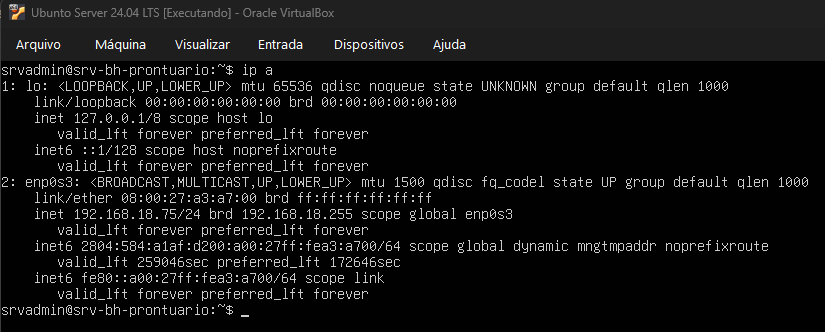
\includegraphics[width=\textwidth]{print_ip_estatico.png}
    \caption{Servidor Ubuntu On-Premise com IP estático configurado (\texttt{192.168.18.75/24})}
    \label{fig:ubuntu_ip}
\end{figure}

\subsection{Servidor Ubuntu (VirtualBox) --- Serviços Ativos}

\begin{figure}[H]
    \centering
    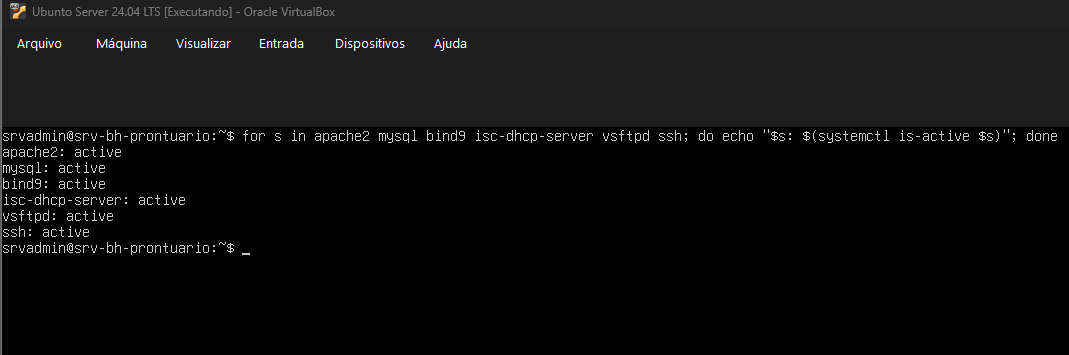
\includegraphics[width=\textwidth]{print_servicos.png}
    \caption{Serviços instalados e ativos no servidor Ubuntu On-Premise}
    \label{fig:ubuntu_servicos}
\end{figure}

\subsection{Instância AWS EC2 --- Nuvem}

\begin{figure}[H]
    \centering
    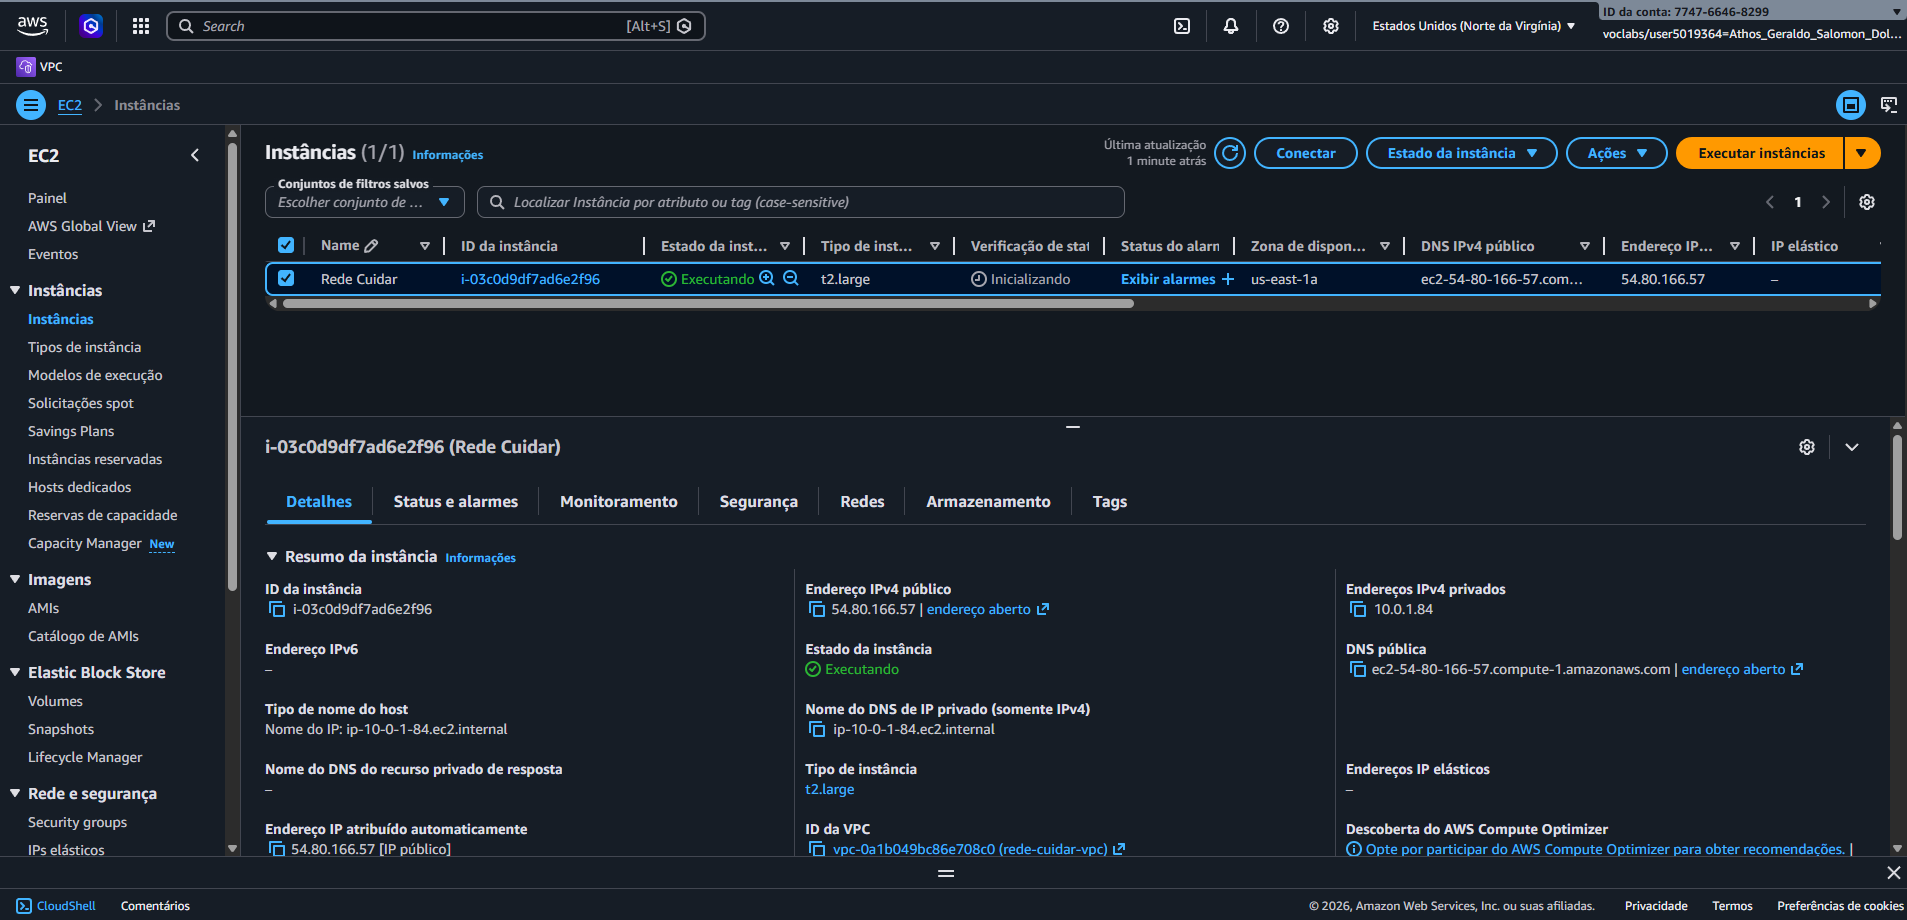
\includegraphics[width=\textwidth]{print_instancia.png}
    \caption{Instância EC2 ``Rede Cuidar'' em execução no painel da AWS}
    \label{fig:aws_instancia}
\end{figure}

\subsection{Windows Server --- Servidor de Aplicação}

\begin{figure}[H]
    \centering
    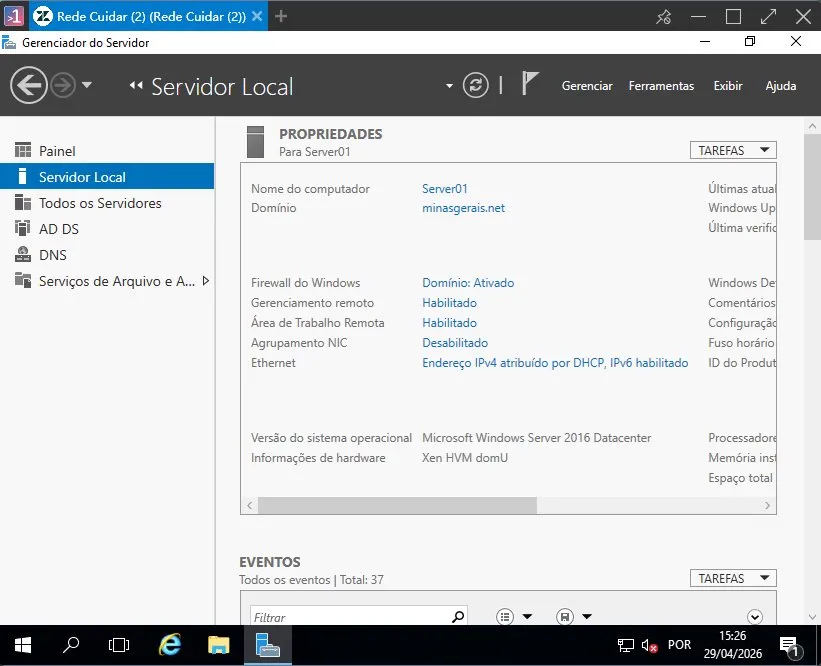
\includegraphics[width=\textwidth]{windows_server.png}
    \caption{Windows Server 2016 Datacenter em execução na instância AWS}
    \label{fig:windows_server}
\end{figure}

\subsection{VPC --- Rede Privada Virtual (AWS)}

\begin{figure}[H]
    \centering
    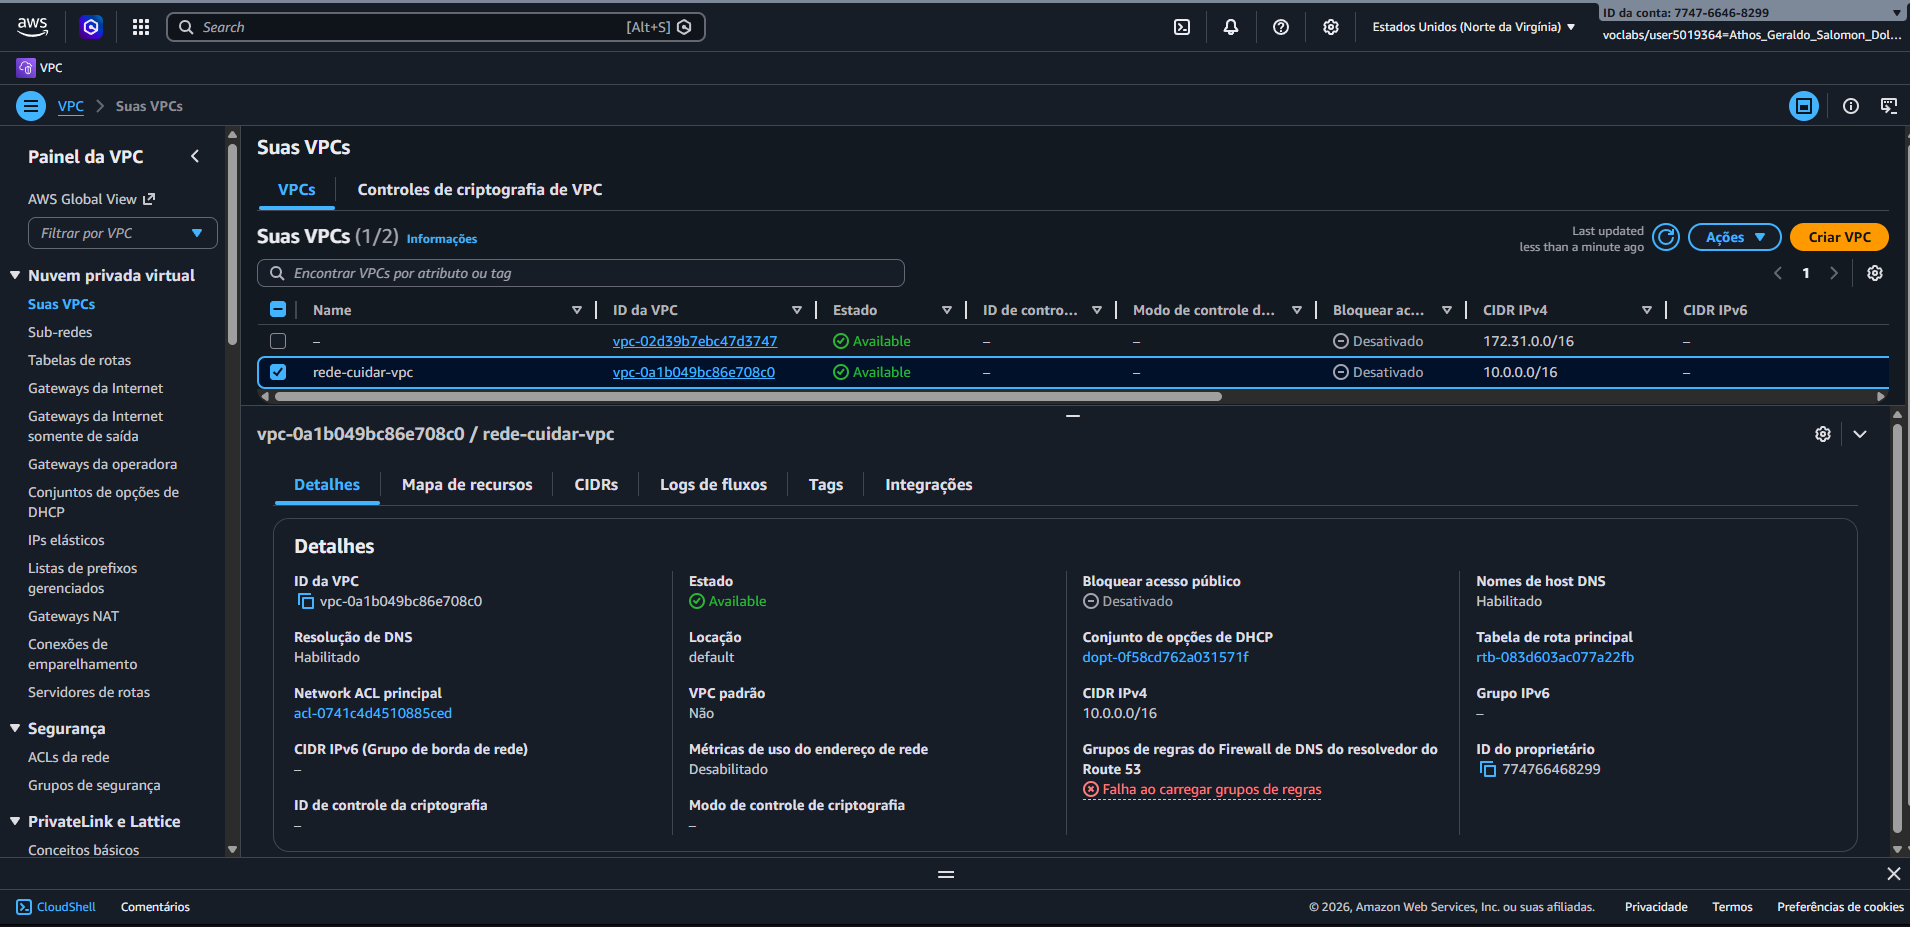
\includegraphics[width=\textwidth]{print_vpc.png}
    \caption{VPC \texttt{rede-cuidar-vpc} configurada na AWS com CIDR \texttt{10.0.0.0/16}}
    \label{fig:vpc}
\end{figure}

\subsection{Active Directory --- Estrutura do Domínio}

\begin{figure}[H]
    \centering
    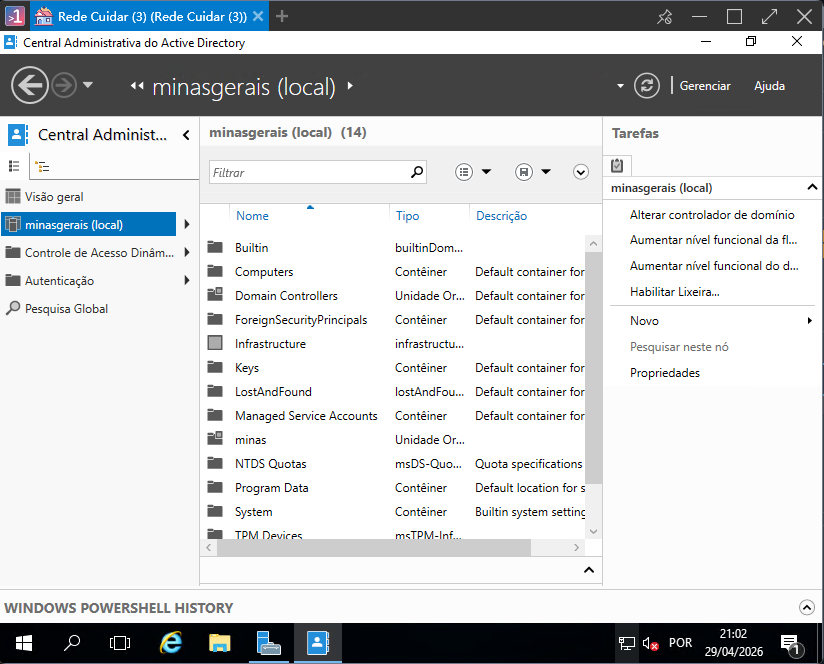
\includegraphics[width=\textwidth]{ad_print.png}
    \caption{Central Administrativa do Active Directory --- domínio \texttt{minasgerais.net}}
    \label{fig:ad_estrutura}
\end{figure}

\subsection{Active Directory --- Unidades Organizacionais (OUs)}

\begin{figure}[H]
    \centering
    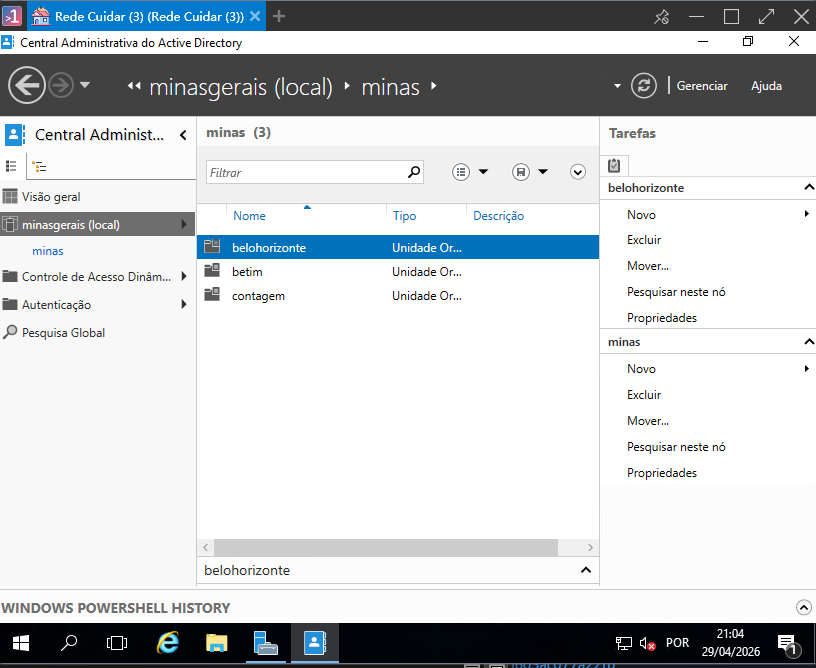
\includegraphics[width=\textwidth]{subredes_print.png}
    \caption{OUs criadas no AD: \texttt{minas} com sub-OUs \texttt{belohorizonte}, \texttt{betim} e \texttt{contagem}}
    \label{fig:ad_ous}
\end{figure}

\subsection{Política de Grupo (GPO)}

\begin{figure}[H]
    \centering
    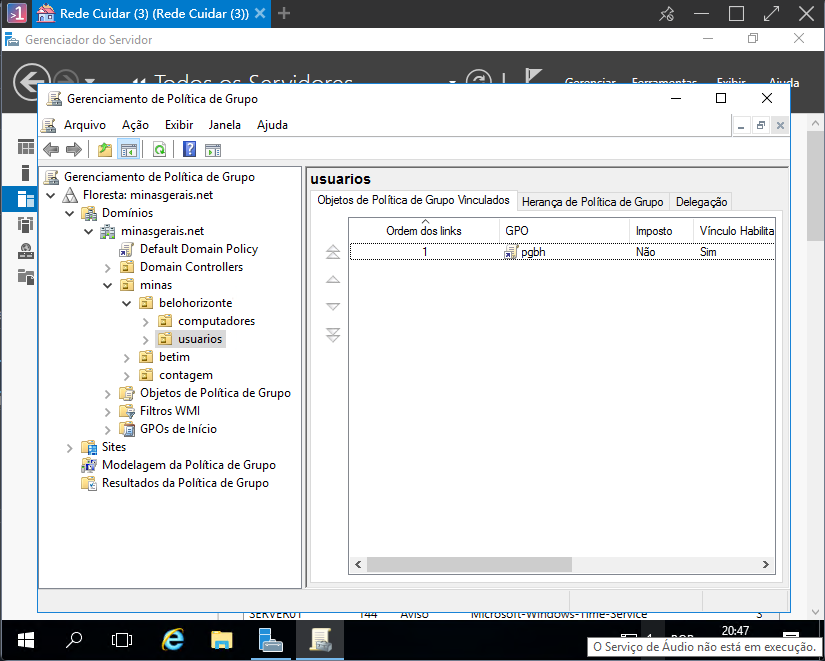
\includegraphics[width=\textwidth]{gpo_criada.png}
    \caption{GPO \texttt{pgbh} vinculada à OU \texttt{usuarios} em \texttt{belohorizonte}}
    \label{fig:gpo}
\end{figure}

\section{Vídeo Demonstrativo}
O vídeo demonstrativo da Etapa 2, exibindo o funcionamento dos ambientes configurados, está disponível no Microsoft Teams pelo link abaixo:

\begin{center}
    \textbf{Link:} \url{https://sgapucminasbr.sharepoint.com/sites/team_sga_2414_2026_1_7378102/_layouts/15/guestaccess.aspx?share=IQBUD9anyHlnSZGWIaAY6TzEAaYO6do7X8C4R6jARODEzeA&e=qDsxRR}
\end{center}

% ============================================================
% ETAPA 3
% ============================================================
\chapter{Etapa 3 --- Monitoramento Ativo da Infraestrutura de Servidores}

\section{Introdução ao Monitoramento Centralizado}
Para garantir os critérios de alta disponibilidade, integridade, identificação proativa de gargalos e comunicação ininterrupta exigidos pela \textbf{Rede Hospitalar Cuidar}, foi consolidada uma solução de monitoramento de ativos utilizando a ferramenta corporativa \textbf{Zabbix}.

Nesta etapa, a infraestrutura foi integrada de ponta a ponta, permitindo a coleta de dados de desempenho em tempo real por meio de agentes dedicados e protocolos de rede. A telemetria abrange o consumo de hardware (processamento, memória, E/S de disco) e volumetria de tráfego de dados, fornecendo visibilidade total sobre o ecossistema local e em nuvem.

\section{Gestão e Organização da Etapa}

\subsection{Responsabilidades e Colaboração}
As atividades da Etapa 3 foram distribuídas entre os membros do grupo conforme as competências demonstradas nas etapas anteriores, garantindo continuidade e coesão na execução do projeto.

\begin{itemize}[label=\color{pucblue}$\bullet$]
    \item \textbf{Igor e Pedro:} Instalação e configuração do Zabbix Appliance como plataforma central de monitoramento, incluindo definição de IP estático e acesso à interface web.
    \item \textbf{Henrique:} Configuração do protocolo SNMP nos servidores Ubuntu e Windows, correção das permissões de acesso no \texttt{snmpd.conf} e cadastro dos hosts no Zabbix.
    \item \textbf{Bernardo e Athos:} Criação do mapa de rede \textit{Rede Hospitalar Cuidar} e configuração do dashboard personalizado com widgets de métricas e alertas.
    \item \textbf{Fabrício:} Análise e interpretação dos dados coletados pelo Zabbix, documentação dos resultados e redação técnica do capítulo.
\end{itemize}

\section{Topologia Lógica e Visões de Gerência}

\subsection{Mapa de Conectividade da Infraestrutura}
Abaixo apresenta-se o mapa de topologia estruturado no painel nativo do Zabbix (\textit{All maps / Rede Hospitalar Cuidar}), ilustrando as relações de conectividade e o fluxo saudável de comunicação entre os nós de gerência.

\begin{figure}[H]
    \centering
    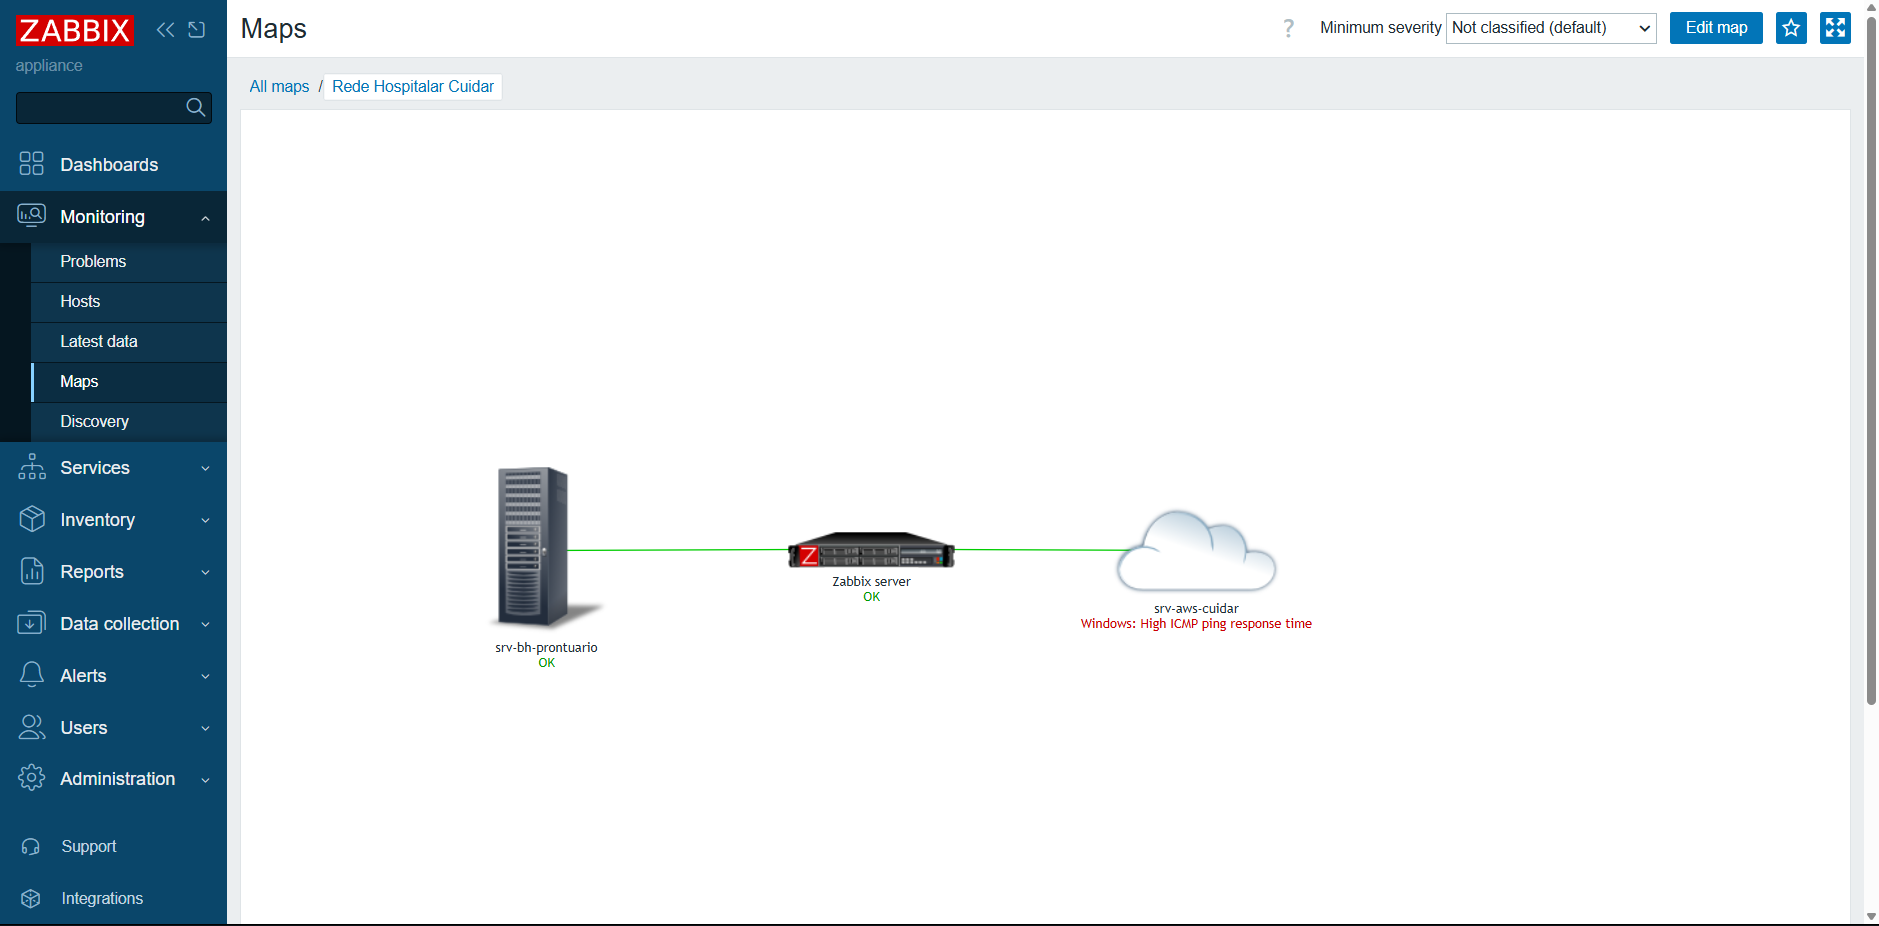
\includegraphics[width=0.9\textwidth]{print_mapa.png}
    \caption{Mapa de monitoramento integrado da infraestrutura local e nuvem no Zabbix}
    \label{fig:zabbix_mapa}
\end{figure}

\subsection{Painel Global de Operações (Dashboard)}
O monitoramento centralizado conta com um painel de controle principal (\textit{Dashboard}), que agrega os principais indicadores de desempenho do ecossistema hospitalar, facilitando a tomada de decisão em nível de suporte de infraestrutura.

\begin{figure}[H]
    \centering
    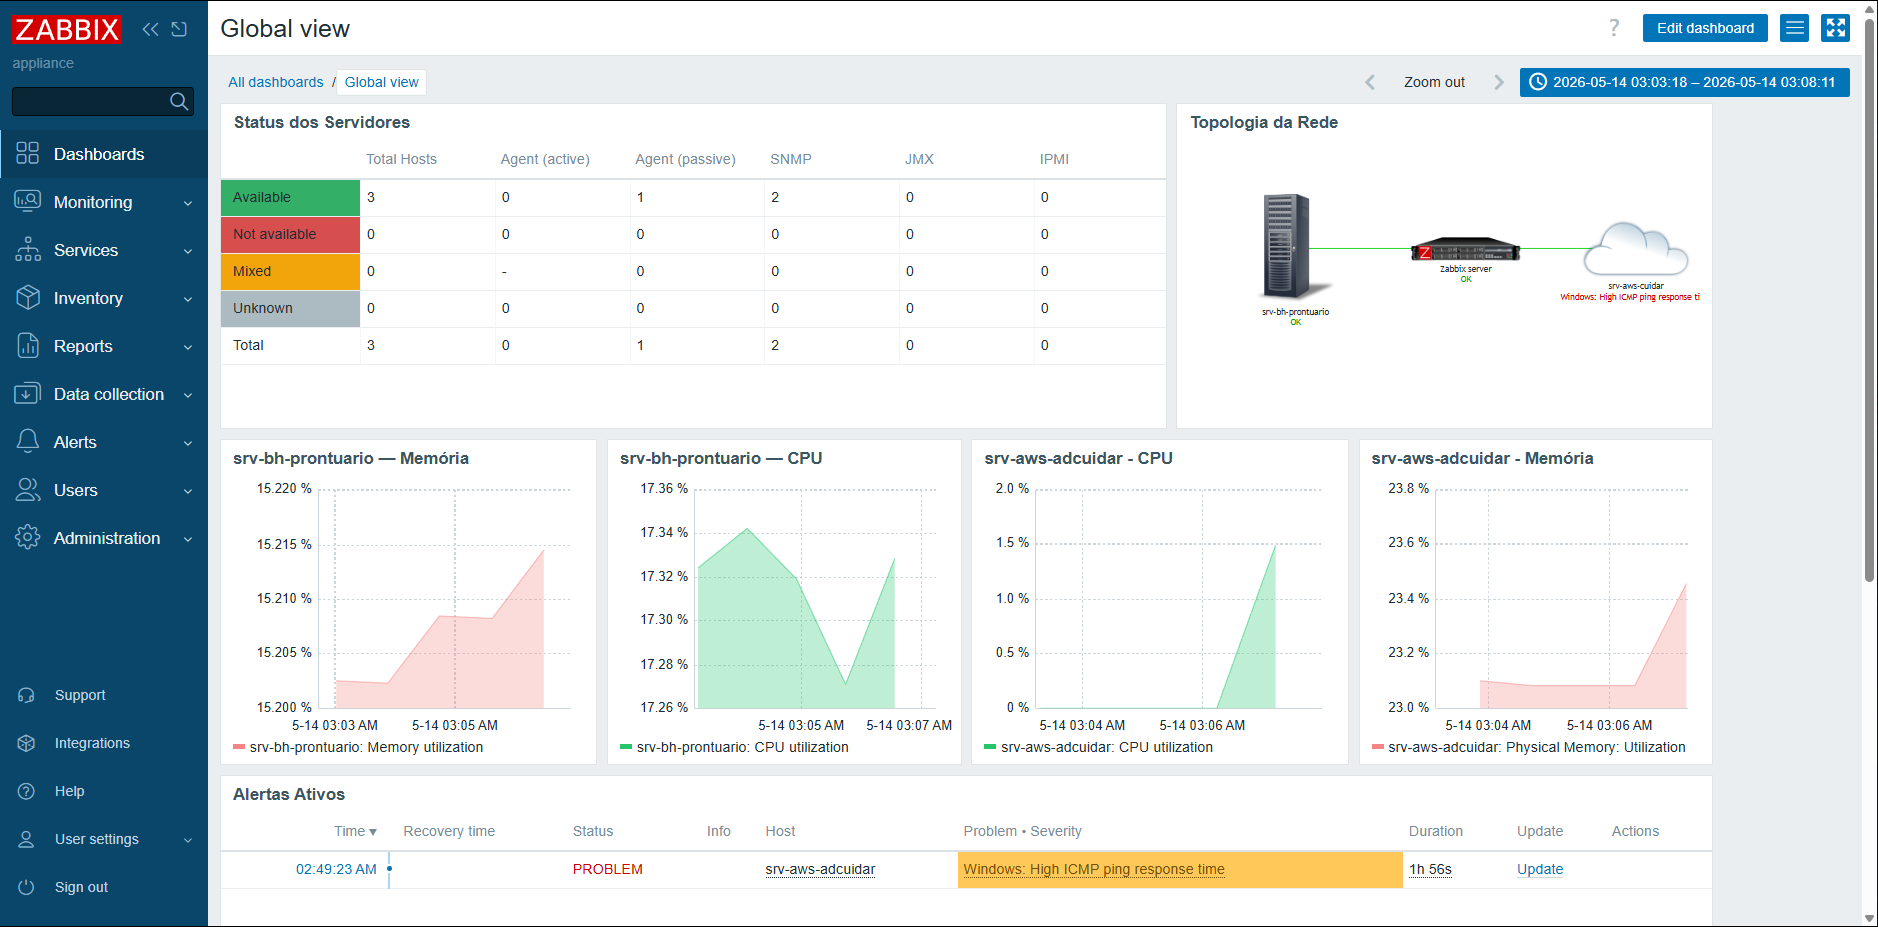
\includegraphics[width=\textwidth]{dashboard_print.png}
    \caption{Dashboard geral do Zabbix exibindo a saúde integrada do ambiente hospitalar}
    \label{fig:zabbix_dashboard}
\end{figure}

\subsection{Inventário de Hosts e Status de Disponibilidade}
Como evidenciado no painel de controle, todos os hosts monitorados foram devidamente parametrizados e encontram-se operando sem a presença de problemas ou alertas ativos. A integração com o agente Zabbix garante a confiabilidade dos status apresentados.

\begin{figure}[H]
    \centering
    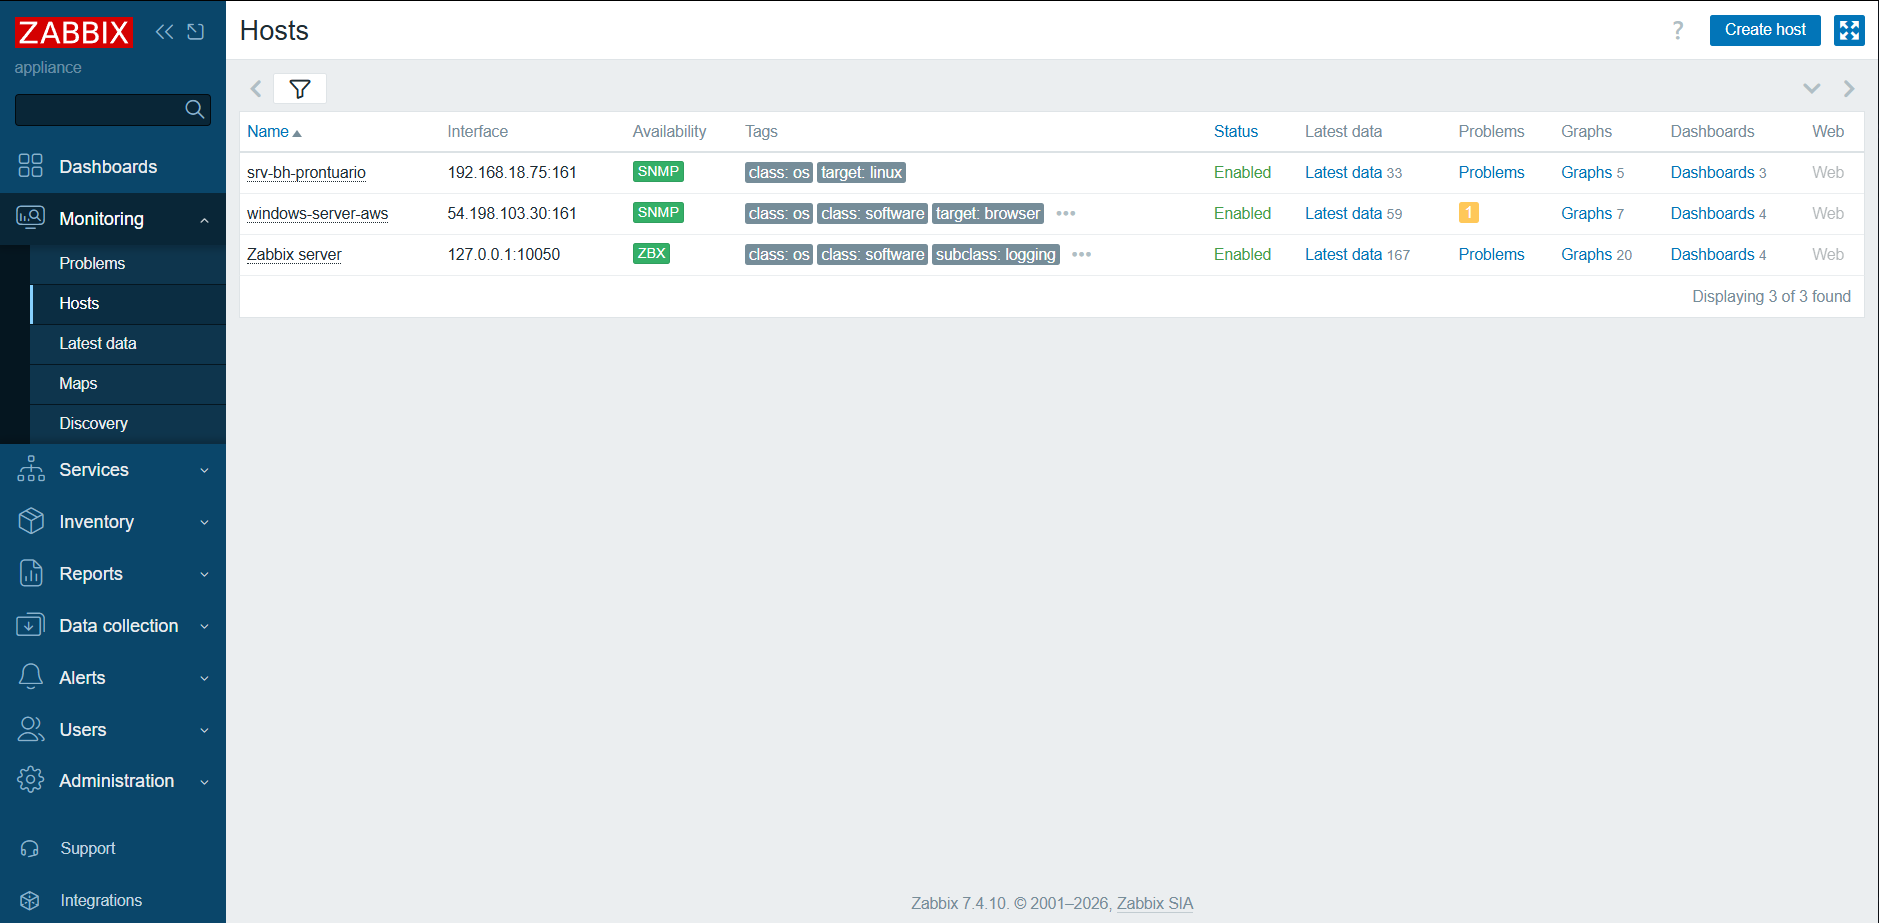
\includegraphics[width=\textwidth]{hosts_verdes.png}
    \caption{Listagem de hosts ativos e com status operacional estabilizado}
    \label{fig:hosts_operacionais}
\end{figure}

\section{Métricas de Performance --- Servidor Local (srv-bh-prontuario)}
O servidor local virtualizado, responsável pelo banco de dados de prontuários eletrônicos e serviços internos da Matriz em Belo Horizonte, teve seu comportamento monitorado e os gráficos gerados comprovam a conformidade do ambiente.

\subsection{Utilização de CPU}
O gráfico ilustra a carga de processamento da CPU do servidor Ubuntu. Nota-se que os níveis operacionais mantêm-se baixos e estáveis, garantindo ampla margem para picos de requisições concorrentes.

\begin{figure}[H]
    \centering
    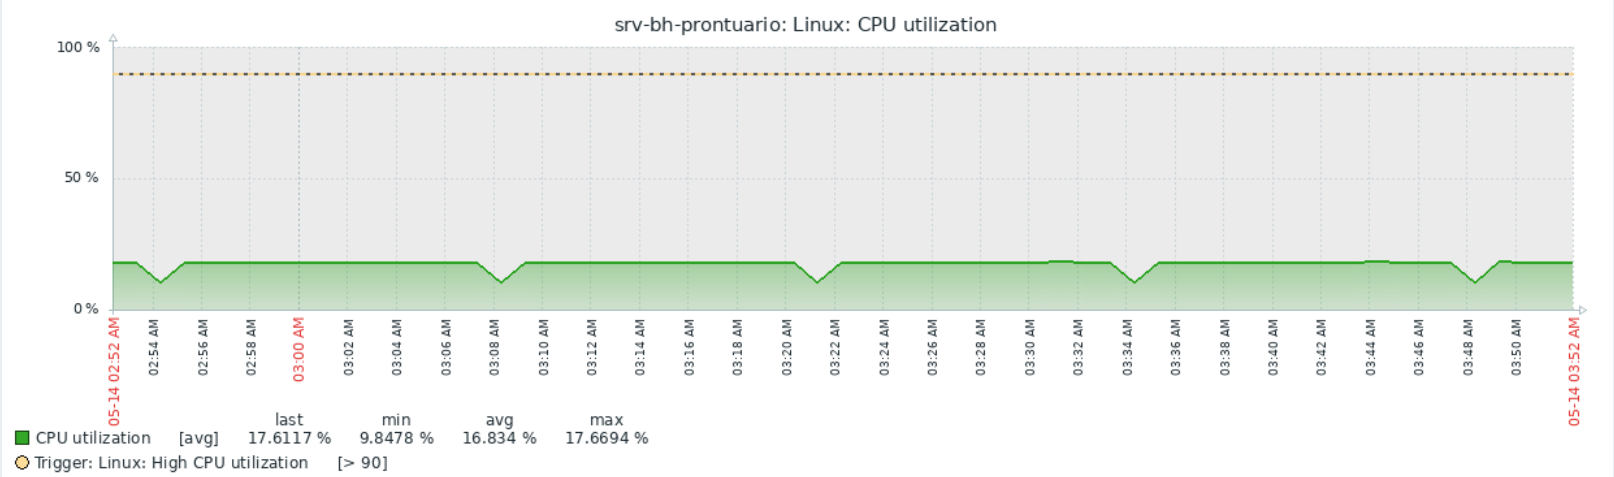
\includegraphics[width=0.9\textwidth]{cpu_utilization_ubuntu.png}
    \caption{Métricas de uso de processador (CPU) no servidor Ubuntu local}
    \label{fig:cpu_ubuntu}
\end{figure}

\subsection{Utilização de Memória RAM}
A telemetria de memória segmenta o espaço total alocado, identificando a fatia utilizada, disponível e em cache, atestando que a máquina não sofre com paginação excessiva em disco.

\begin{figure}[H]
    \centering
    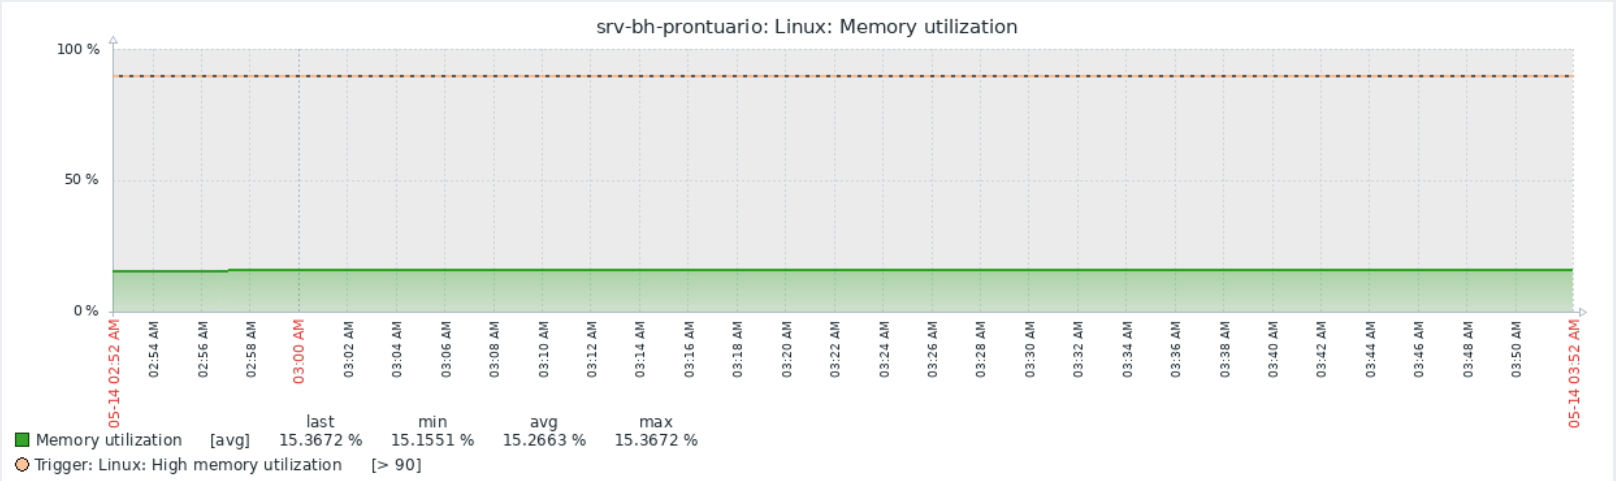
\includegraphics[width=0.9\textwidth]{memory_utilization_ubuntu.png}
    \caption{Análise de alocação e consumo de memória RAM do servidor local}
    \label{fig:memoria_ubuntu}
\end{figure}

\subsection{E/S de Disco (Leitura e Escrita)}
Monitorar as operações de entrada e saída por segundo (IOPS) e taxa de transferência é crucial para o banco de dados MySQL. O gráfico confirma baixa latência de gravação física.

\begin{figure}[H]
    \centering
    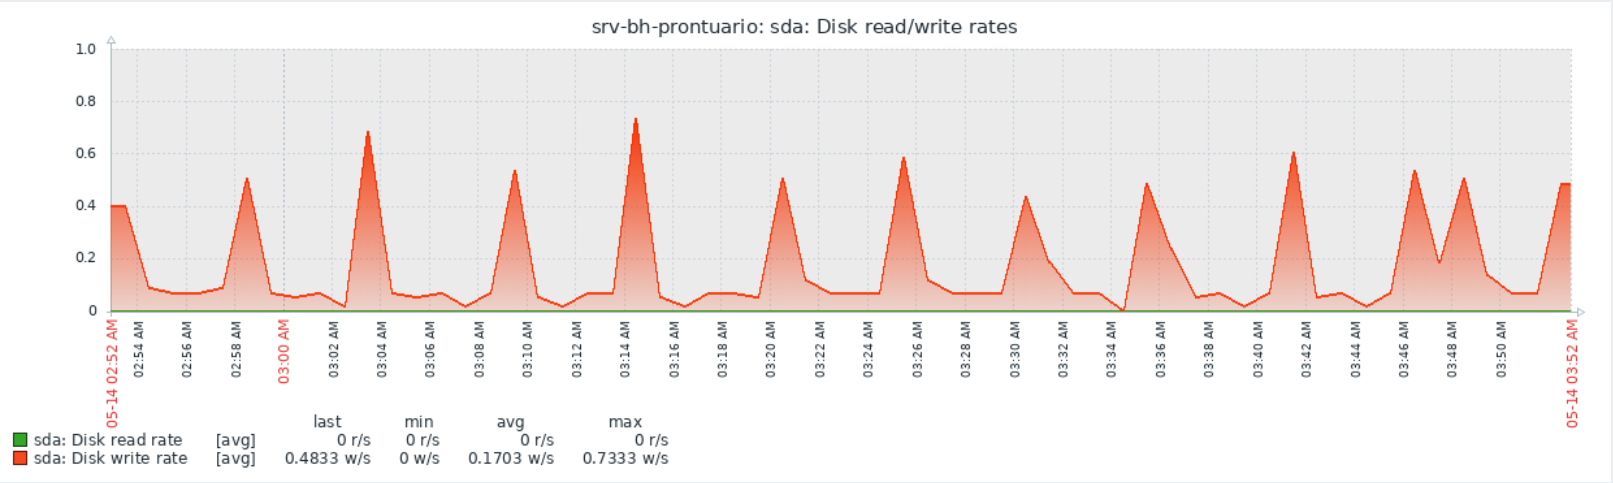
\includegraphics[width=0.9\textwidth]{disco_readwirte_ubuntu.png}
    \caption{Estatísticas de leitura e escrita em disco do servidor de banco de dados}
    \label{fig:disco_ubuntu}
\end{figure}

\subsection{Tráfego de Rede}
O volume de dados trafegado pela interface de rede (\texttt{enp0s3}) exibe o fluxo simétrico de dados de entrada (\textit{In}) e saída (\textit{Out}), atestando a integridade das respostas do Apache2 e DNS BIND9.

\begin{figure}[H]
    \centering
    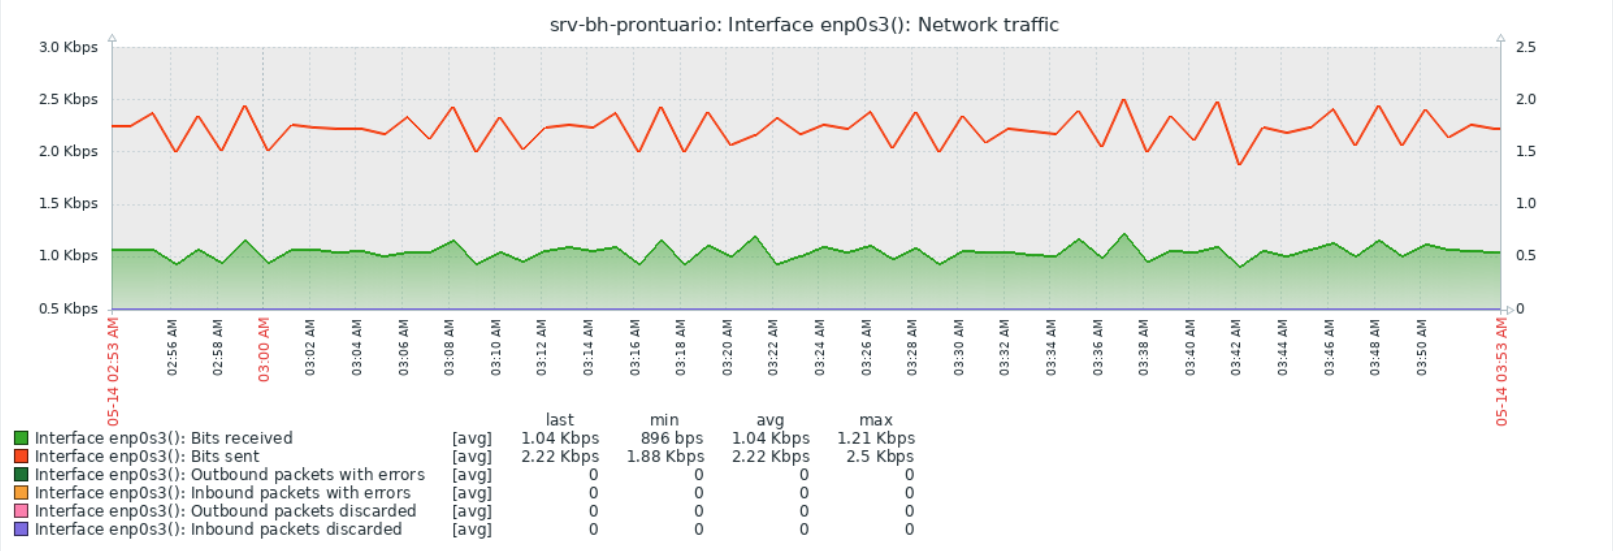
\includegraphics[width=0.9\textwidth]{network_traffic_ubuntu.png}
    \caption{Volume e taxa de transferência de pacotes na interface de rede local}
    \label{fig:rede_ubuntu}
\end{figure}

\section{Métricas de Performance --- Servidor em Nuvem (srv-aws-cuidar)}
A instância EC2 alocada na região de Norte da Virgínia (\texttt{us-east-1}), que atua com o papel de controlador de domínio Active Directory e hospedagem do back-end hospitalar, teve suas métricas consolidadas.

\subsection{Utilização de CPU}
O monitoramento via contador do Windows Server mapeia as flutuações de uso do processador da instância \texttt{t2.large}. Os dados coletados apontam para um comportamento saudável e livre de gargalos lógicos de processamento.

\begin{figure}[H]
    \centering
    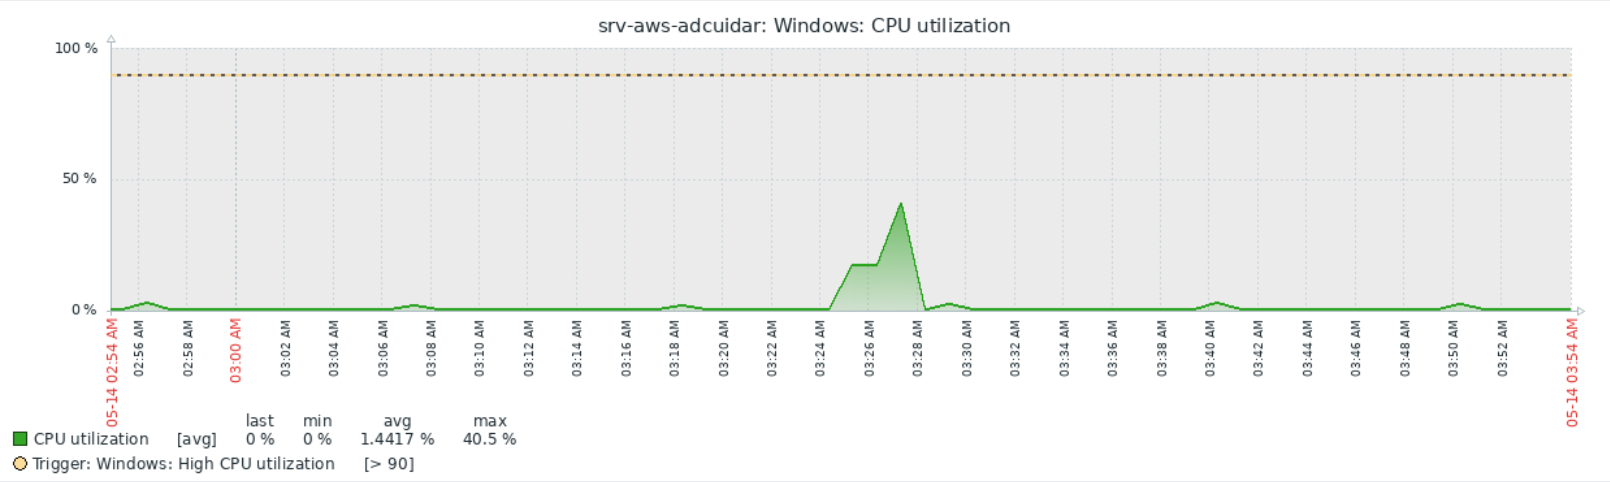
\includegraphics[width=0.9\textwidth]{cpu_utilization_aws.png}
    \caption{Métricas de processamento da instância EC2 Windows Server na AWS}
    \label{fig:cpu_aws}
\end{figure}

\subsection{Utilização de Memória RAM}
A telemetria exibe o consumo percentual e em bytes da memória do Windows Server. O gráfico assegura que o Active Directory e as políticas de grupo (GPO) aplicadas estão rodando de forma otimizada.

\begin{figure}[H]
    \centering
    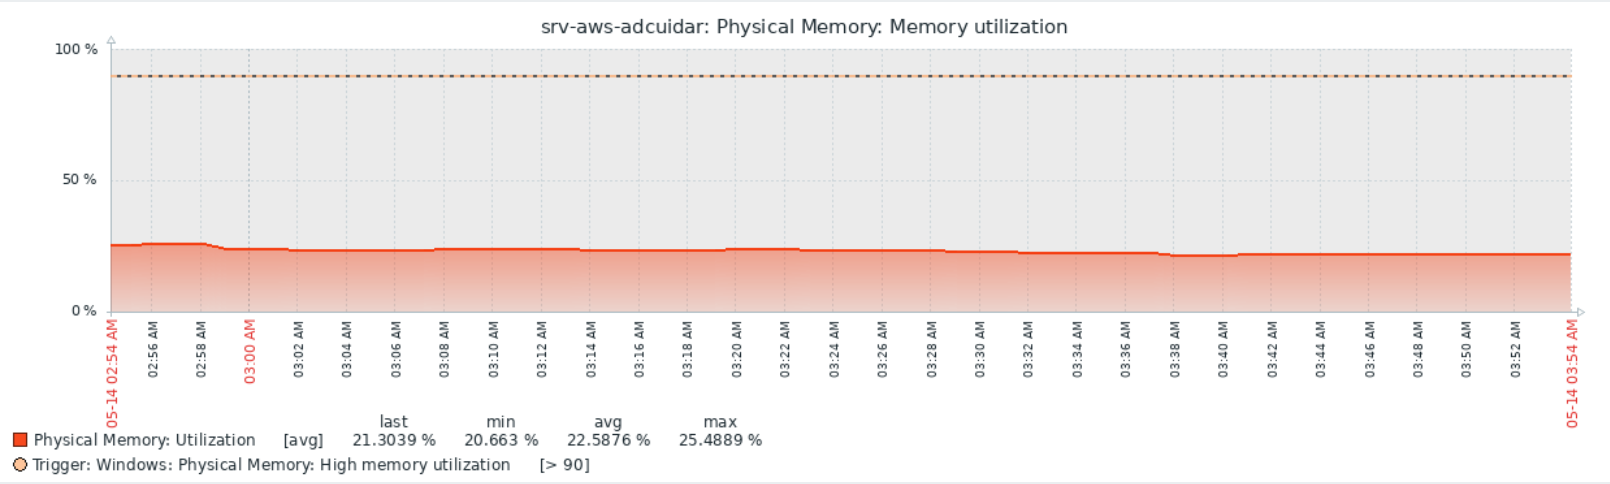
\includegraphics[width=0.9\textwidth]{memory_utilization_aws.png}
    \caption{Gráfico de uso de memória física na instância de aplicação em nuvem}
    \label{fig:memoria_aws}
\end{figure}

\subsection{Tráfego de Rede na Instância Cloud}
Os dados exibem o tráfego que cruza a placa de rede virtual conectada à VPC. A estabilidade dos gráficos comprova que, após a parametrização fina dos limiares (\textit{thresholds}) de checagem do Zabbix, a latência geográfica maior devido à rota internacional foi devidamente mitigada, não interferindo na qualidade da coleta contínua de dados do agente.

\begin{figure}[H]
    \centering
    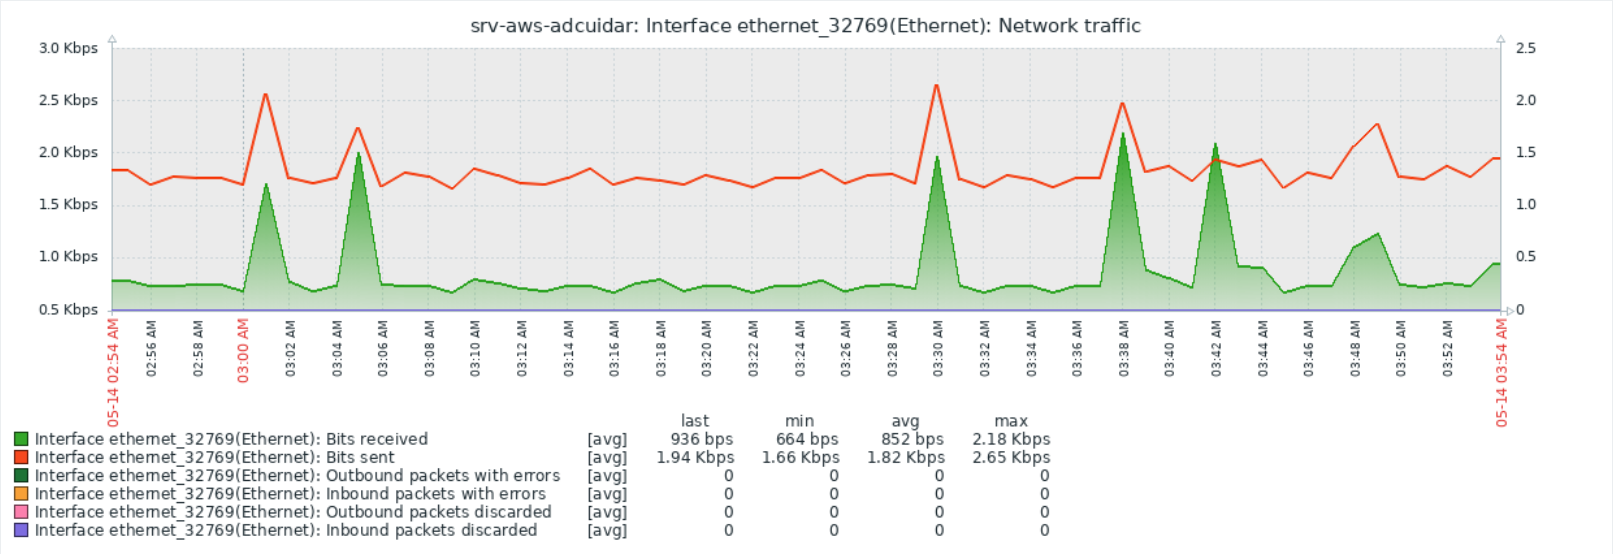
\includegraphics[width=0.9\textwidth]{rede_utilization_aws.png}
    \caption{Análise de pacotes enviados e recebidos através da interface WAN da AWS}
    \label{fig:rede_aws}
\end{figure}

% ============================================================
% ETAPA 4
% ============================================================
\chapter{Etapa 4 --- Segurança da Informação e Aplicação Back-End}

\section{Introdução}

A Etapa 4 do projeto da Rede Hospitalar Cuidar teve como objetivo fortalecer os aspectos relacionados à segurança da informação da infraestrutura desenvolvida nas etapas anteriores. Além da elaboração da Política de Segurança da Informação (PSI), foi desenvolvida uma aplicação web para gerenciamento de pacientes, bem como uma cartilha de conscientização voltada aos colaboradores da organização.

Adicionalmente, foram realizadas análises de vulnerabilidades do ambiente implantado, permitindo identificar riscos potenciais e propor mecanismos de mitigação alinhados às boas práticas recomendadas pelo OWASP Top 10 e às exigências da Lei Geral de Proteção de Dados (LGPD).

\section{Política de Segurança da Informação}

Com o objetivo de estabelecer diretrizes formais para proteção dos ativos de informação da organização, foi elaborada a Política de Segurança da Informação (PSI) da Rede Hospitalar Cuidar.

O documento foi desenvolvido com base nas recomendações da norma ABNT NBR ISO/IEC 27001 e contempla princípios fundamentais de confidencialidade, integridade e disponibilidade das informações.

Entre os principais tópicos abordados pela política destacam-se:

\begin{itemize}[label=\color{pucblue}$\bullet$]
    \item Controle de acesso e autenticação;
    \item Segurança física e ambiental;
    \item Proteção das redes e comunicações;
    \item Gestão de incidentes de segurança;
    \item Programas de treinamento e conscientização;
    \item Avaliação contínua dos mecanismos de segurança;
    \item Conformidade com requisitos legais e regulatórios.
\end{itemize}

A PSI estabelece responsabilidades para todos os colaboradores da instituição e define procedimentos para garantir a proteção das informações sensíveis manipuladas pela organização.

\section{Cartilha de Boas Práticas de Acesso Seguro}

Complementando a Política de Segurança da Informação, foi desenvolvida uma cartilha de boas práticas destinada aos colaboradores da Rede Hospitalar Cuidar.

A cartilha foi elaborada em linguagem acessível, buscando conscientizar os usuários sobre os principais riscos de segurança presentes no ambiente corporativo.

Os assuntos abordados incluem:

\begin{itemize}[label=\color{pucblue}$\bullet$]
    \item Criação e utilização segura de senhas;
    \item Identificação de tentativas de phishing;
    \item Engenharia social;
    \item Cuidados no tratamento dos dados dos pacientes;
    \item Procedimentos de reporte de incidentes;
    \item Recomendações para acesso remoto seguro.
\end{itemize}

A adoção dessas práticas contribui para reduzir riscos operacionais e fortalecer a cultura de segurança da informação dentro da organização.

\section{Aplicação Web para Gestão de Pacientes}

Como parte das entregas desta etapa, foi desenvolvida uma aplicação web para gerenciamento de pacientes da Rede Hospitalar Cuidar.

A solução foi implementada utilizando o framework Flask em conjunto com o banco de dados MySQL, permitindo a realização das operações fundamentais de um sistema CRUD (\textit{Create, Read, Update and Delete}).

Entre as funcionalidades implementadas destacam-se:

\begin{itemize}[label=\color{pucblue}$\bullet$]
    \item Cadastro de pacientes;
    \item Consulta dos registros armazenados;
    \item Atualização das informações cadastradas;
    \item Exclusão de pacientes;
    \item Associação dos pacientes às unidades de atendimento da rede.
\end{itemize}

A aplicação foi disponibilizada tanto no ambiente local quanto no ambiente em nuvem, permitindo validar a integração entre os serviços de infraestrutura implementados ao longo do projeto.

\section{Evidências da Aplicação Desenvolvida}

A Figura \ref{fig:tela_inicio} apresenta a página inicial do sistema da Rede Hospitalar Cuidar.

\begin{figure}[H]
\centering
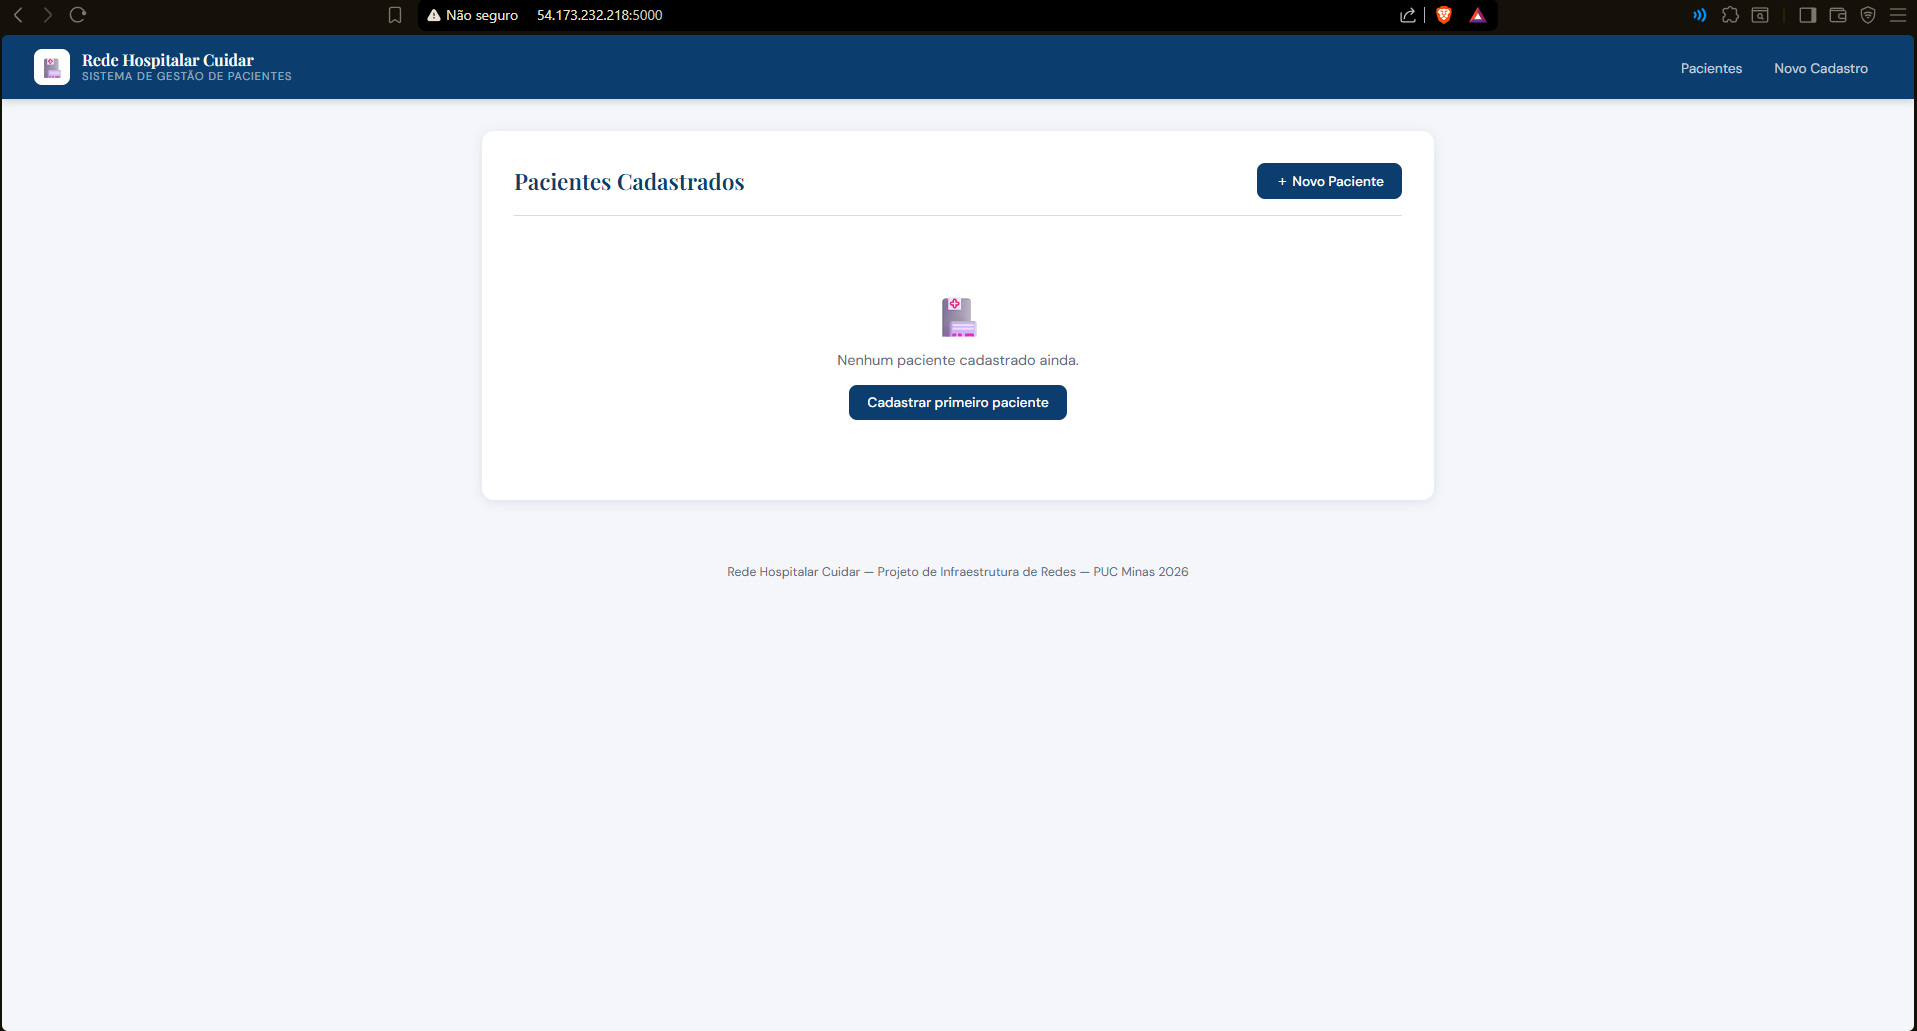
\includegraphics[width=\textwidth]{tela_de_inicio.png}
\caption{Tela inicial da aplicação de gerenciamento de pacientes.}
\label{fig:tela_inicio}
\end{figure}

A Figura \ref{fig:cadastro_paciente} apresenta a tela utilizada para realizar o cadastro de novos pacientes.

\begin{figure}[H]
\centering
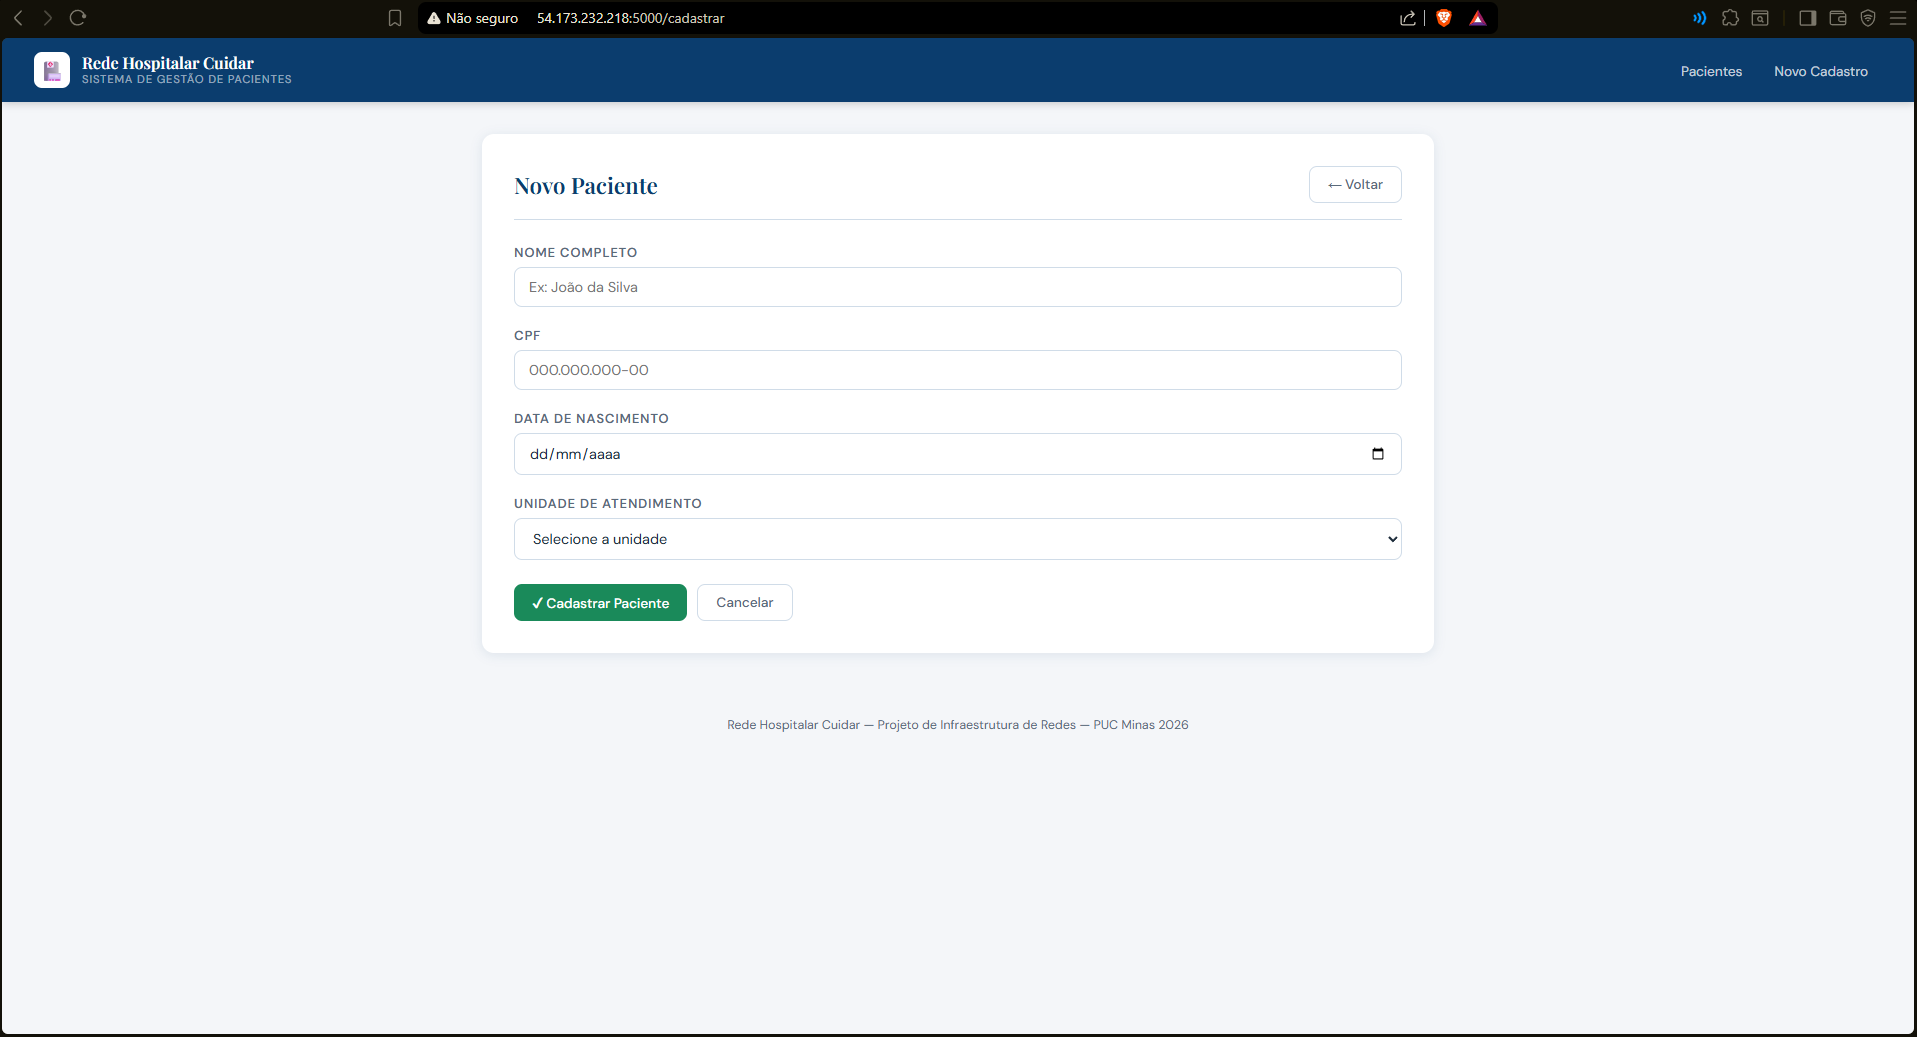
\includegraphics[width=\textwidth]{cadastro_de_pacientes.png}
\caption{Formulário de cadastro de pacientes.}
\label{fig:cadastro_paciente}
\end{figure}

Após o cadastro, os pacientes passam a ser exibidos na listagem principal da aplicação, conforme mostrado na Figura \ref{fig:pacientes_cadastrados}.

\begin{figure}[H]
\centering
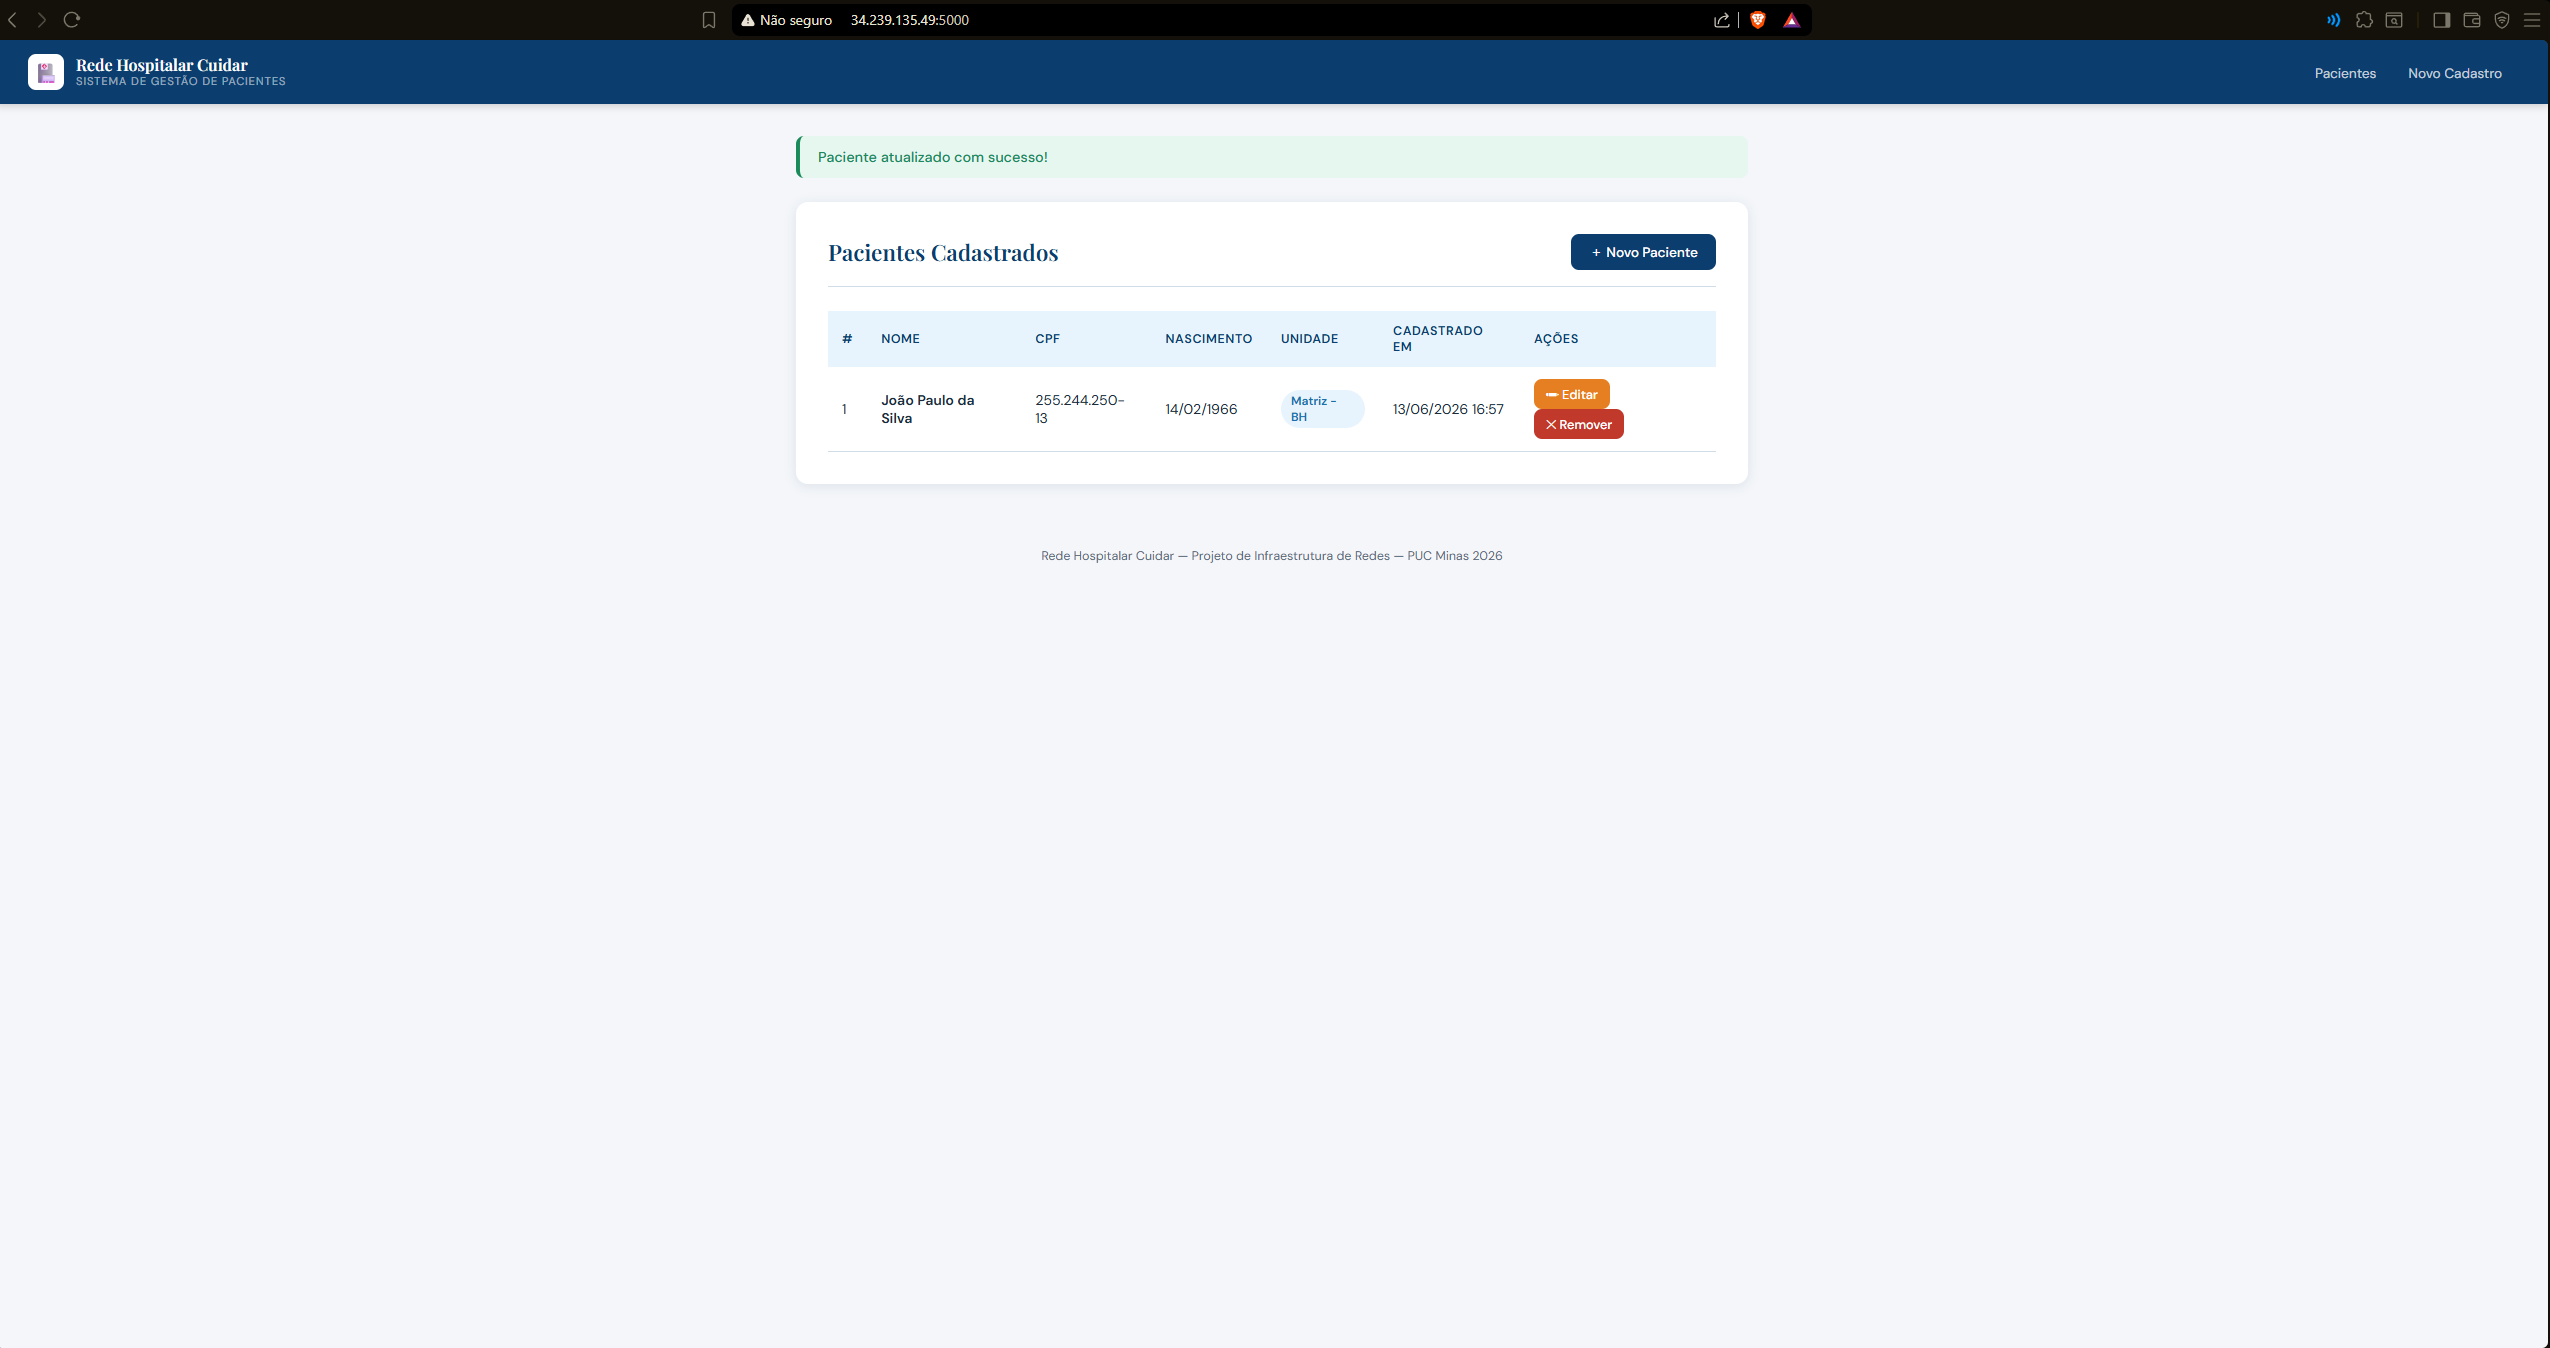
\includegraphics[width=\textwidth]{paciente_cadastrado.png}
\caption{Listagem dos pacientes cadastrados no sistema.}
\label{fig:pacientes_cadastrados}
\end{figure}

A funcionalidade de edição das informações dos pacientes é apresentada na Figura \ref{fig:editar_paciente}.

\begin{figure}[H]
\centering
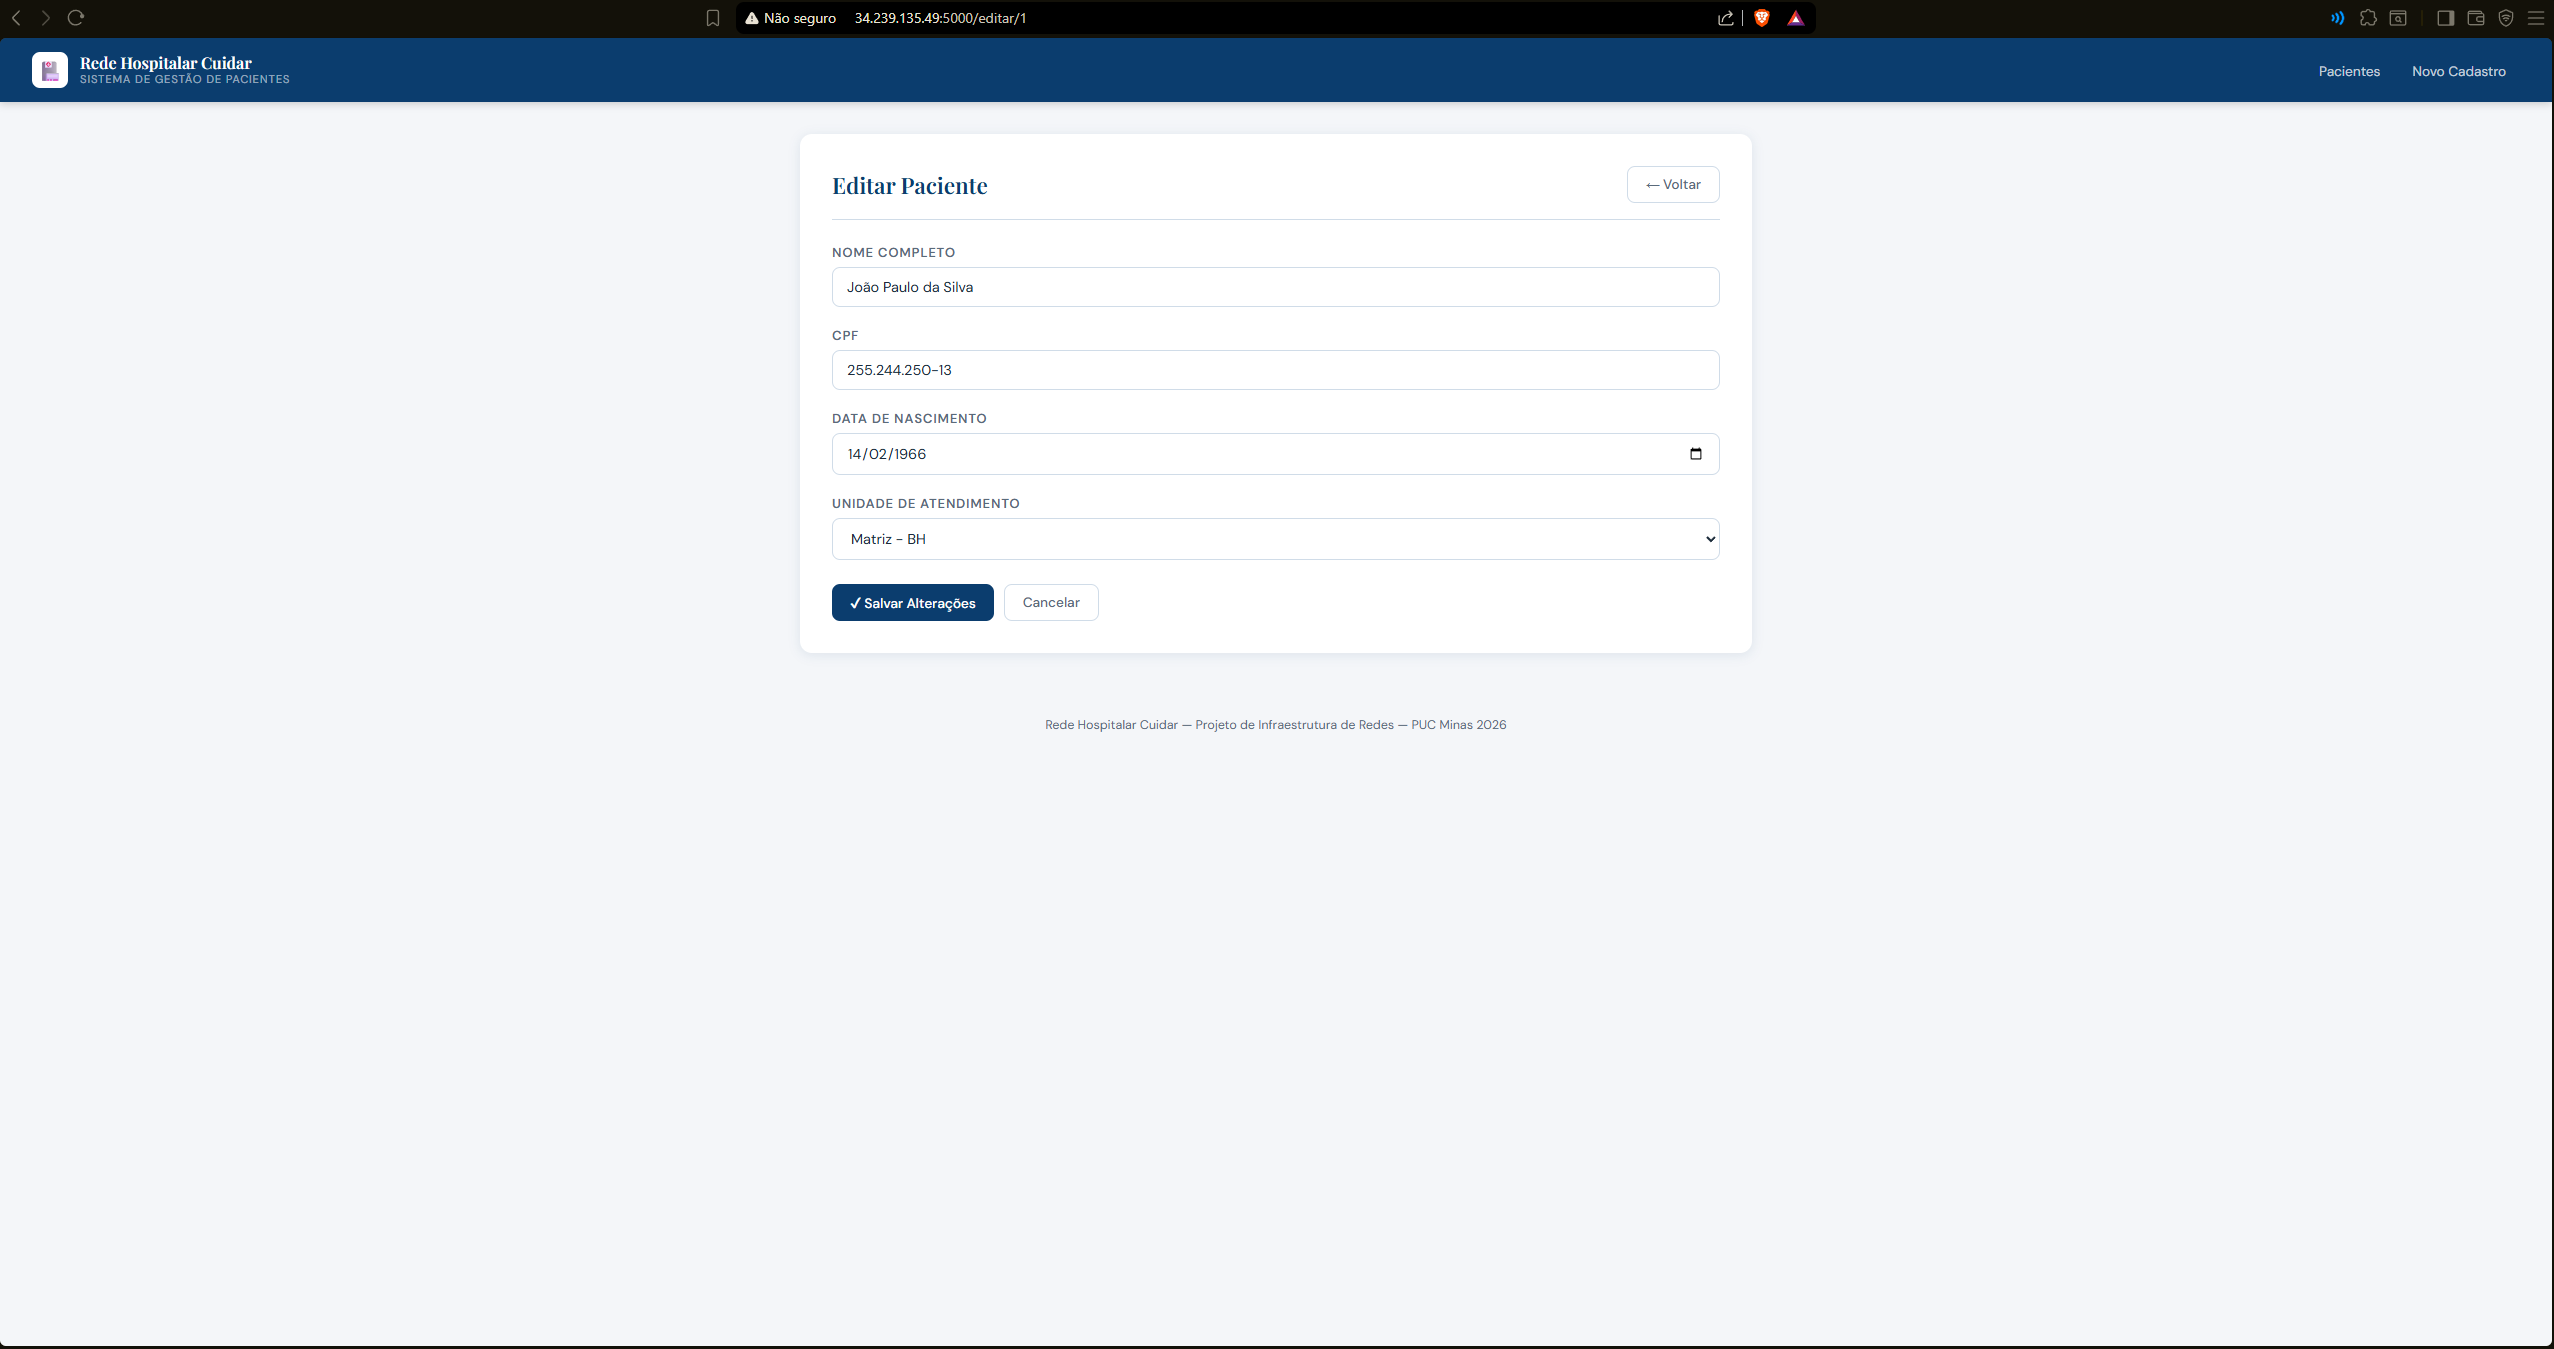
\includegraphics[width=\textwidth]{editar_paciente.png}
\caption{Tela de edição dos dados de um paciente.}
\label{fig:editar_paciente}
\end{figure}

\section{Análise de Vulnerabilidades}

Com base na infraestrutura implantada para hospedar a aplicação da Rede Hospitalar Cuidar, foram identificadas três vulnerabilidades classificadas segundo o OWASP Top 10 (2021).

\subsection{Injeção de SQL (SQL Injection)}

A aplicação recebe informações por meio dos formulários HTML e realiza operações sobre o banco de dados MySQL. Caso consultas parametrizadas não sejam utilizadas adequadamente em todas as rotas da aplicação, existe a possibilidade de exploração por meio de ataques de SQL Injection.

Como medida mitigadora, recomenda-se a utilização exclusiva de consultas parametrizadas (\textit{prepared statements}) e a aplicação do princípio do menor privilégio aos usuários do banco de dados.

\subsection{Ausência de Criptografia das Comunicações}

A aplicação encontra-se acessível por meio do protocolo HTTP, sem utilização de TLS.

Essa característica permite que os dados trafeguem em texto puro, possibilitando ataques de interceptação e comprometendo a confidencialidade das informações dos pacientes.

Como solução, recomenda-se a utilização de um proxy reverso Nginx associado a certificados digitais TLS, permitindo a utilização do protocolo HTTPS.

\subsection{Ausência de Controle de Acesso e Autenticação}

Foi identificado que a aplicação não implementa mecanismos de autenticação e autorização.

Dessa forma, qualquer usuário que possua acesso ao endereço da aplicação pode visualizar, alterar ou excluir registros de pacientes.

Como medida corretiva, recomenda-se a implementação de autenticação baseada em sessões utilizando Flask-Login, associada a um modelo RBAC (\textit{Role Based Access Control}), permitindo diferentes níveis de permissão conforme o perfil do usuário.

\section{Divisão das Atividades da Etapa}

As atividades da Etapa 4 foram distribuídas entre os integrantes do grupo de acordo com suas competências e disponibilidade, garantindo a entrega de todos os artefatos previstos para esta fase do projeto.

\begin{itemize}[label=\color{pucblue}$\bullet$]
    \item \textbf{Athos Geraldo Salomon Dolabela da Silveira:} Participou da elaboração da Política de Segurança da Informação (PSI), do desenvolvimento da aplicação web em Flask, da configuração do banco de dados MySQL e da implantação da solução tanto no servidor local quanto no ambiente em nuvem utilizando instância EC2 com IP elástico.

    \item \textbf{Pedro Tolentino Gontijo:} Participou da elaboração da Política de Segurança da Informação, da revisão da documentação produzida e prestou suporte ao desenvolvimento e à implantação da aplicação no ambiente computacional.

    \item \textbf{Bernardo Elias Renttins Vasconcelos de Sousa:} Responsável pela elaboração e pelo design da cartilha de boas práticas de acesso seguro destinada aos colaboradores da Rede Hospitalar Cuidar.

    \item \textbf{Henrique Fadel Carvalho:} Participou da elaboração e revisão da cartilha de boas práticas, contribuindo para adequar a linguagem utilizada ao público não técnico da organização.

    \item \textbf{Igor de Oliveira Martins dos Santos:} Responsável pela redação e estruturação do relatório técnico da etapa, pela documentação do ambiente implantado e pela análise das vulnerabilidades identificadas.

    \item \textbf{Fabrício Junio da Silva:} Participou da redação e revisão do relatório técnico, além de colaborar na documentação das vulnerabilidades e das entregas realizadas durante a etapa.
\end{itemize}

\section{Conclusão da Etapa 4}

A Etapa 4 permitiu consolidar os mecanismos de segurança da informação da Rede Hospitalar Cuidar, integrando aspectos técnicos e organizacionais.

Além da elaboração da Política de Segurança da Informação e da cartilha de conscientização, foi desenvolvida e implantada uma aplicação web para gerenciamento de pacientes, demonstrando a integração entre infraestrutura, banco de dados e desenvolvimento de software.

Por fim, a análise das vulnerabilidades possibilitou identificar pontos de melhoria e propor mecanismos de mitigação alinhados às recomendações do OWASP Top 10 e às exigências da LGPD, contribuindo para aumentar a maturidade de segurança da solução implementada.




% ============================================================
% ETAPA 5
% ============================================================
\chapter{Etapa 5 --- Elaboração da Apresentação Final do Projeto}

\section{Objetivo da Etapa}

A quinta etapa do projeto teve como objetivo consolidar os resultados obtidos ao longo do desenvolvimento da infraestrutura da Rede Hospitalar Cuidar em uma apresentação final, permitindo a exposição organizada das soluções implementadas e dos resultados alcançados pelo grupo.

A apresentação foi desenvolvida utilizando a plataforma Overleaf, por meio da classe \textit{Beamer} em \LaTeX, possibilitando a elaboração colaborativa do material e a padronização visual dos slides.

\section{Organização e Colaboração da Equipe}

Seguindo a metodologia de trabalho adotada nas etapas anteriores, todos os integrantes participaram ativamente da construção da apresentação, sendo responsáveis pela elaboração dos slides referentes às atividades que desenvolveram durante o projeto.

A distribuição das atividades ocorreu de forma colaborativa, permitindo que cada membro contribuísse com a organização do conteúdo e com a revisão do material produzido.

\begin{itemize}[label=\color{pucblue}$\bullet$]

\item \textbf{Igor de Oliveira Martins dos Santos e Pedro Tolentino Gontijo:} elaboração dos slides referentes ao planejamento da infraestrutura e aos serviços em nuvem;

\item \textbf{Henrique Fadel Carvalho:} preparação dos conteúdos relacionados à virtualização, Active Directory e configuração dos servidores;

\item \textbf{Bernardo Elias Renttins Vasconcelos de Sousa e Athos Geraldo Salomon Dolabela da Silveira:} organização visual da apresentação, inserção das evidências e revisão do material;

\item \textbf{Fabrício Junio da Silva:} revisão textual, padronização da documentação e organização da sequência lógica dos slides.

\end{itemize}

\section{Estrutura da Apresentação}

A apresentação foi organizada de forma a representar cronologicamente as etapas do projeto, abordando:

\begin{enumerate}

\item Planejamento da infraestrutura da Rede Hospitalar Cuidar;

\item Implantação do ambiente em nuvem e virtualização local;

\item Configuração dos serviços e do Active Directory;

\item Monitoramento da infraestrutura por meio do Zabbix;

\item Aplicação das práticas de segurança da informação;

\item Demonstração da aplicação CRUD desenvolvida para gerenciamento de pacientes;

\item Principais vulnerabilidades identificadas e recomendações de mitigação;

\item Conclusões gerais do projeto.

\end{enumerate}

\section{Resultados Obtidos}

A evolução da apresentação permitiu consolidar todos os conhecimentos desenvolvidos ao longo do semestre, reunindo em um único material as evidências, resultados e soluções implementadas para a Rede Hospitalar Cuidar.

Além disso, a atividade proporcionou maior integração entre os membros da equipe, contribuindo para a organização do conteúdo e para a preparação da apresentação final do projeto perante a disciplina.

\section{Conclusão da Etapa 5}

Com a conclusão desta etapa, foi possível sintetizar em uma única apresentação os principais artefatos produzidos durante o desenvolvimento do projeto, facilitando a comunicação dos resultados alcançados e evidenciando a integração entre os conhecimentos de infraestrutura de redes, computação em nuvem, monitoramento, segurança da informação e desenvolvimento de aplicações.

A construção colaborativa dos slides também reforçou a participação de todos os integrantes da equipe, contribuindo para a preparação da apresentação final e para a consolidação dos conhecimentos adquiridos ao longo da disciplina.



\chapter*{Conclusão Geral do Projeto}
\addcontentsline{toc}{chapter}{Conclusão Geral do Projeto}

O desenvolvimento do projeto da Rede Hospitalar Cuidar permitiu consolidar, de forma integrada, os conhecimentos adquiridos ao longo da disciplina de Infraestrutura de Redes. A solução proposta contemplou todas as etapas necessárias para o planejamento, implementação, monitoramento e proteção de um ambiente corporativo híbrido voltado ao setor de saúde.

A infraestrutura projetada foi estruturada com segmentação lógica de redes, serviços locais e em nuvem, controle centralizado por meio do Active Directory, monitoramento contínuo com Zabbix e mecanismos de segurança alinhados às recomendações da LGPD e do OWASP Top 10.

Além dos aspectos relacionados à infraestrutura, o projeto incorporou o desenvolvimento de uma aplicação web para gerenciamento de pacientes, demonstrando a integração entre redes, banco de dados, computação em nuvem e desenvolvimento de software.

Os resultados obtidos evidenciam que a solução atende aos requisitos de disponibilidade, escalabilidade, segurança e gerenciamento centralizado, contribuindo para a modernização dos processos da Rede Hospitalar Cuidar.

\chapter*{Referências}
\addcontentsline{toc}{chapter}{Referências}



AMAZON WEB SERVICES. \textbf{Visão geral da Amazon Web Services: Whitepaper da AWS}. 2024. Disponível em: \url{https://docs.aws.amazon.com/pt_br/whitepapers/latest/aws-overview/aws-overview.pdf}. Acesso em: 17 jun. 2026.

\vspace{0.2cm}

ASSOCIAÇÃO BRASILEIRA DE NORMAS TÉCNICAS. \textbf{ABNT NBR ISO/IEC 27001: Tecnologia da informação --- técnicas de segurança --- sistemas de gestão da segurança da informação --- requisitos}. Rio de Janeiro: ABNT, 2013.

\vspace{0.2cm}

BRASIL. \textbf{Lei n. 12.965, de 23 de abril de 2014: Marco Civil da Internet}. Brasília: Diário Oficial da União, 2014. Disponível em: \url{https://www.planalto.gov.br/ccivil_03/_ato2011-2014/2014/lei/l12965.htm}. Acesso em: 17 jun. 2026.

\vspace{0.2cm}

BRASIL. \textbf{Lei n. 13.709, de 14 de agosto de 2018: Lei Geral de Proteção de Dados Pessoais (LGPD)}. Brasília: Diário Oficial da União, 2018. Disponível em: \url{https://www.planalto.gov.br/ccivil_03/_ato2015-2018/2018/lei/l13709.htm}. Acesso em: 17 jun. 2026.

\vspace{0.2cm}

CARDOSO, W. L. L.; ROCHA, S. D. \textbf{Estudo de caso sobre a infraestrutura de redes e o impacto em pacientes em estado de UTI}. Revista FT, v. 29, n. 146, 2025. Disponível em: \url{https://revistaft.com.br/estudo-de-caso-sobre-a-infraestrutura-de-redes-e-o-impacto-em-pacientes-em-estado-de-uti/}. Acesso em: 17 jun. 2026.

\vspace{0.2cm}

CONSELHO FEDERAL DE MEDICINA. \textbf{Resolução CFM n. 1.821/2007: Normas técnicas para digitalização e uso dos sistemas informatizados para a guarda e manuseio dos prontuários dos pacientes}. Brasília: CFM, 2007.

\vspace{0.2cm}

FLASK. \textbf{Flask Documentation (3.x)}. 2024. Disponível em: \url{https://flask.palletsprojects.com}. Acesso em: 17 jun. 2026.

\vspace{0.2cm}

GIL, A. C. \textbf{Como elaborar projetos de pesquisa}. 7. ed. Barueri: Atlas, 2022.

\vspace{0.2cm}

MICROSOFT. \textbf{Documentação do Active Directory Domain Services}. Redmond: Microsoft Corporation, 2024. Disponível em: \url{https://learn.microsoft.com/pt-br/windows-server/identity/ad-ds/active-directory-domain-services}. Acesso em: 17 jun. 2026.

\vspace{0.2cm}

OWASP FOUNDATION. \textbf{OWASP Top Ten 2021}. 2021. Disponível em: \url{https://owasp.org/www-project-top-ten/}. Acesso em: 17 jun. 2026.

\vspace{0.2cm}

RODRIGUES, G. B. et al. \textbf{Zabbix na TI hospitalar: eficiência operacional e cuidado ao paciente}. Revista Esfera Acadêmica Tecnologia, v. 9, n. 1, 2024. ISSN 2526-4141. Disponível em: \url{https://multivix.edu.br/wp-content/uploads/2024/10/REVISTA_ESFERA_TECNOLOGIA_V09_N01_ARTIGO2.pdf}. Acesso em: 17 jun. 2026.

\vspace{0.2cm}

TAVARES, M. H.; CORREIA, M. F. C.; SOARES, G. L. \textbf{A computação em nuvem como solução estratégica: comparação de ferramentas e análise dos benefícios e desafios para infraestruturas de TI}. 2025. Monografia (Sistemas de Informação) --- Pontifícia Universidade Católica de Minas Gerais, Unidade São Gabriel, Belo Horizonte, 2025. Disponível em: \url{https://bib.pucminas.br/pergamumweb/download/B53DB2A1-8659-4C5C-84CF-1BA86CB889CA.pdf}. Acesso em: 17 jun. 2026.

\vspace{0.2cm}

WAZLAWICK, R. S. \textbf{Metodologia de pesquisa para ciência da computação}. 3. ed. Rio de Janeiro: LTC, 2021.

\vspace{0.2cm}

ZABBIX SIA. \textbf{Manual do Zabbix}. 2024. Disponível em: \url{https://www.zabbix.com/documentation/current/pt/manual}. Acesso em: 17 jun. 2026.




% O comando abaixo DEVE ser a última linha do arquivo main.tex

\end{document}